\documentclass[12pt, a4paper,twoside]{tesi_upf}
\renewcommand{\baselinestretch}{1.3}

\usepackage{tikz}

\usepackage{float}

\usepackage{pdfpages}

\usepackage{color}
\usepackage{subfigure}


\usetikzlibrary{shapes.geometric, arrows}

\tikzstyle{startstop} = [rectangle, rounded corners, minimum width=3cm, minimum height=1cm,text centered, draw=black, fill=red!30]

\tikzstyle{io} = [trapezium, trapezium left angle=70, trapezium right angle=110, minimum width=3cm, minimum height=1cm, text centered, draw=black, fill=blue!30]

\tikzstyle{process} = [rectangle, minimum width=3cm, minimum height=1cm, text centered, text width=3cm, draw=black, fill=orange!30]

\tikzstyle{decision} = [diamond, minimum width=3cm, minimum height=1cm, text centered, draw=black, fill=green!30]

\tikzstyle{arrow} = [thick,->,>=stealth]

%CODIFICACIÓ
\usepackage[utf8]{inputenc}


%IDIOMES
\usepackage[catalan,english]{babel}

%NOMÉS PER A OBTENIR INDICACIÓ DEL MARC EN MIDA A4
%\usepackage[cam,a4,center,frame]{crop}

%PER A INCLOURE GRÀFICS I EL LOGO DE LA UPF
\usepackage{graphicx}
\newsavebox\IBoxA \newsavebox\IBoxB \newlength\IHeight
\newcommand\TwoFig[6]{% Image1 Caption1 Label1 Image2 ...
  \sbox\IBoxA{\includegraphics[width=0.45\textwidth]{#1}}
  \sbox\IBoxB{\includegraphics[width=0.45\textwidth]{#4}}%
  \ifdim\ht\IBoxA>\ht\IBoxB
    \setlength\IHeight{\ht\IBoxB}\else\setlength\IHeight{\ht\IBoxA}\fi%
  \begin{figure}[H]
  \minipage[t]{0.45\textwidth}\centering
  \includegraphics[height=\IHeight]{#1}
  \caption{#2}\label{#3}
  \endminipage\hfill
  \minipage[t]{0.45\textwidth}\centering
  \includegraphics[height=\IHeight]{#4}
  \caption{#5}\label{#6}
  \endminipage 
  \end{figure}%
}
%!htb
\usepackage{caption}
\usepackage{acronym}
\usepackage{multirow}
%FONTS TIMES O GARAMOND, 
\usepackage{times}
%\usepackage{garamond}
\usepackage[hyphens]{url}
\usepackage{hyperref}

\usepackage{pdfpages}
%SENSE HEADINGS: NO MODIFICAR
\pagestyle{plain}

%PER A L'ÍNDEX DE MATÈRIES
\usepackage{makeidx}
\makeindex

%ESTIL DE BIBLIOGRAFIA
\bibliographystyle{apalike}


%AQUEST DOCUMENT ÉS EN CATALÀ
\selectlanguage{english}

%EN COMPTES DE ÍNDEX, LA TAULA DE CONTINGUTS ES TITULA SUMARI
\addto\captionscatalan
  {\renewcommand{\contentsname}{\Large \sffamily Sumari}}

% ~~~~~~~~~~~~~~~~~~~~~~~~~~
% CUSTOM PACKAGES
% ~~~~~~~~~~~~~~~~~~~~~~~~~~
\usepackage[hidelinks]{hyperref}
\usepackage{titlesec}
\setcounter{secnumdepth}{4}
\usepackage{pdfpages}
\usepackage{cite}

%AFEGIU EN AQUESTA PART LES VOSTRES DADES
\title{Visual Interface for Wi-Fi Networks Monitoring}
\author{Ferran Selva Rodríguez}
\thyear{2014}
\department{Departament de Tecnologies de la Informació i les Comunicacions (DTIC)}
\supervisor{Jaume Barceló}


\begin{document}

\pdfstringdefDisableCommands{%
\let\MakeUppercase\relax
}

\frontmatter

\maketitle

\cleardoublepage


%%%%%% Dedicatòria; si no es vol posar, comenteu fins a final de dedicatòria

\noindent This document is dedicated to my parents, Paqui and Manel, and my brother Pau, who always gave me their support and estimation.

\cleardoublepage

%%%%%% Final de dedicatòria


%%%%%% Agraïments; si no es vol posar, comenteu fins a final de agraïments
\noindent {\Large \sffamily Acknowledgments}
\\[12pt] 
I want to thank my pilot supervisor, Jaume Barceló, for his
guidance and patience. His support boosted me to perform and complete these thesis.

Also, I want to thank to my department partners, Sergio Almendros, Pedro Vílchez and Iván Fernandez who always have helped me, during this thesis elaboration. 

Thanks to Dani Valderas, Alejandro Juez, Carles Xavier Vilás and Jacob Uribe for your work and support during these years of classes, labs and deliverables.
\cleardoublepage

%%%%%% Final dels agraïments

%ABSTRACT EN DOS IDIOMES. COM A MÍNIM CATALÀ. SI L'ALTRE ÉS EN CASTELLA CANVIEU EL QUE POSA ABSTRACT
\selectlanguage{english}
\section*{\Large \sffamily Abstract}
The open Wi-Fi, at the city, is increasingly used by the citizens.
Barcelona, a city with more than 720 Wi-Fi access points, and an average of 66.912 users in 2013, is an example. Under this scenario, currently growing, this project aims at offering a web visualization of the availability of access points of a Wi-Fi access network. Two examples of such access networks are \emph{BarcelonaWi-Fi} and \emph{Poblenou Sense Fils}. The tool is general enough to be used in other access networks. 

This tool is divided in two parts. The first one is a Raspberry Pi that directly connects to the Wi-Fi access network and continuously gathers data about the availability of the access points. This information is sent to the second part, which is a server with a NoSQL database and a web interface to visualize the data on a map.

The ultimate goal is to increase the visibility and transparency of the Wi-Fi services offered to the citizenship and encourage citizen participation in improving these services.

\selectlanguage{catalan}
\vspace*{\fill}
\section*{\Large \sffamily  Resum}

El Wi-Fi obert, a la ciutat és cada vegada més utilitzat pels ciutadans. 
Barcelona, una ciutat amb més de 720 punts d'accés Wi-Fi, i una mitjana de 66.912 usuaris el 2013, és un exemple. Sota aquest escenari, actualment en creixement, aquest projecte té com a objectiu oferir una visualització web de la disponibilitat dels punts d'accés d'una xarxa d'accés Wi-Fi. Dos exemples d'aquestes xarxes d'accés són \emph{BarcelonaWi-Fi} i \emph{Poblenou Sense Fils}. L'eina és prou general per ser utilitzada en altres xarxes d'accés. 

Aquesta eina es divideix en dues parts. La primera és una Raspberry Pi que es connecta directament a la xarxa d'accés Wi-Fi i contínuament recull dades sobre la disponibilitat dels punts d'accés. Aquesta informació s'envia a la segona part, que és un servidor amb una base de dades NoSQL i una interfície web per visualitzar les dades en un mapa. 

L'objectiu final és augmentar la visibilitat i la transparència dels serveis de Wi-Fi que s'ofereix a la ciutadania i fomentar la participació ciutadana en la millora d'aquests serveis.


\vspace*{\fill}

\selectlanguage{english}
\cleardoublepage
%FIN DE ABSTRACTE

%PREFACI OPCIONAL. SI NO ES VOL, COMENTEU FINS EL FINAL DE PREFACI
%{\bf Prefaci}
%
%\cleardoublepage
%FINAL DE PREFACI


%TAULA DE CONTINGUTS: OBLIGATÒRIA
\selectlanguage{english}
\tableofcontents

%INDEX DE FIGURES; NOMÉS ES POSA SI HI HA FIGURES
\listoffigures
%Fa que aparegui al sumari
\addcontentsline{toc}{chapter}{List of figures}

%INDEX DE TAULES; NOMÉS ES POSA SI HI HA TAULES
\listoftables
%Fa que aparegui al sumari
\addcontentsline{toc}{chapter}{List of tables}


%COMENÇA EL TEXT
\mainmatter
\chapter{Introduction}
\label{Chapter1}

This thesis is part of a new way of acting in terms of the provision of Internet services. This new tendency is BuB, Bottom-up-Broadband, which provides a new way of design, deploy and operate networks where the main actions to be carried out are promoted by the user \cite{bubu}.

Until now, Internet Service Providers (ISP) were responsible of the Internet regarding design, deployment and operation of the network, in which they remain completely owners of the infrastructure to provide the service. Now with this new form of network deployment, end users are the owners of the network, and therefore responsible of its consumption and maintenance.

This thesis aims at providing a tool to monitor the status of the access points of "\emph{Barcelona WiFi}" and share this information with the citizens. To gather the information from "\emph{Barcelona WiFi}" access points, the collaboration of the Institut Municipal d'Informàtica (IMI) is required. The tool is general enough to be used by other Wi-Fi access networks in Barcelona and other cities.


The project consists of two parts, the part of collecting data of the \emph{Barcelona WiFi} access points, and the part of representing the data collected in such way that the ordinary citizen can benefit from this information. 

To carry out this project, it is needed two devices, a server and a Raspberry PI. In addition, it requires programming a web service and a web application and the configuration of the server. It is needed too, to program a software for the generation, transfer and storage of the hotspots information, which is located at the Raspberry PI.

The elements of this system, and its operation, are explained at the following chapters.
  
\chapter{State of the Art}
\label{Chapter2}

Wi-Fi is a wireless technology with a limited range, emerged from the wireless communication incompatibility existed between devices from different manufacturers.

This incompatibility made that a group of companies of this sector, found an association with the aim of define the behavior that would use wireless technology to act on and connect, making it consistent between brands. 

This association is Wi-Fi Alliance, whose mission, nowadays, is to check and validate the products interoperability and the standard security protections. An example of its functions is to certificate the products that meet 802.11 \cite{wifialliance}.

The usage of public Wi-Fi is growing. The data proves it. In 2013, there has been an increase in the number of public hotspots, reaching the 6.3 million. Also, it is estimated that during the 2013, the 70\% of the mobile users, browsed once a week using these hotspots \cite{informe2013}.

Forecasts for 2017, say that 12 million public hotspots will be reached, 93\% more than in 2013, while users of public Wi-Fi will exceed 3.300 million. Likewise, it is expected that in 2017, 8 out of 10 cellphones will browse using public Wi-Fi, absorbing 60\% of the mobile data traffic \cite{informe2013}. 

The main reasons of this success are, the lower costs, the higher speed, and the increasing reliability of these type of networks \cite{informe2013}.

Given these data, we can see how the Wi-Fi will be a widely used tool in telecommunications, and for this reason, its control and monitoring will allow institutions, or entities responsible of these networks know how are these networks used. This is a vital aspect in the world of the future.

\section{GOWEX}
Gowex, is a telecommunication company, based in Madrid, Spain, whose activity is to deploy Wi-Fi networks for the cities. These networks, are similar to the networks deployed by the cities council, like \emph{Barcelona WiFi}. The main difference between these networks is the network owner. The owner of public Wi-Fi networks, usually, is the council, but in this case, the owner is a private company. And a second difference is that the GOWEX network, has a free service, but has a payment option too, that give a better service for those who need better features. This option is not available in networks deployed by city councils.

Gowex area of coverage extends over 80 cities worldwide, including cities like Madrid, New York or Miami. Madrid is the european city with more coverage. There are more than 3000 access points installed in Madrid streets and buildings \cite{gowex1}.

\subsection{Wireless Smart City}
The wireless smart cities are cities with full Wi-Fi coverage for all citizens, where the services given to the citizens are improved using Wi-Fi networks. Samples of this mesure are semaphore control management or the control of transport fleets. These tools not only improve the services offered to the citizen, additionally, reduce ordinary day-to-day costs.

\section{MONITORING SOFTWARE}

There are programs for monitoring networks to obtain information from network nodes. These programs use protocols such as SNMP, ICMP or TCP. 

Some of these programs are:
\subsection{Pandora FMS}
Pandora FMS is an open source monitoring software. This software supports protocols such as ICMP, SNMP o TCP, and includes geolocation feature since version 3.1. There is an enterprise version of this software, that has better features and options. Pandora FMS is developed by Spanish company Ártica Soluciones Tecnológicas \cite{pandorafms}.

        \begin{figure}[H]
          \centering
              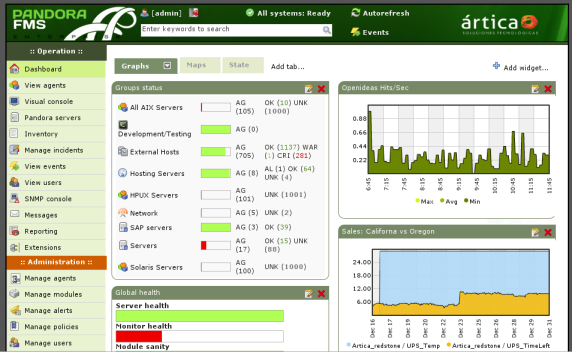
\includegraphics[scale=0.9]{./figures/PandoraFMS.png}
              \rule{32em}{0.5pt}
          \caption[Pandora FMS]{Pandora FMS.}
          \label{fig:Pandora}
        \end{figure}

\subsection{PRTG Network Monitor}
PRTG Network Monitor is a monitoring software developed by Paessler AG. 
Some of this software functionalities are:
\begin{itemize}
\item Uptime/Downtime monitoring.
\item Bandwidth monitoring, using SNMP, WMI and others.
\item SLA monitoring.
\item QoS monitoring.
\item Flexible alerts.
\end{itemize}

This company, specialized in network monitoring and testing, has other software tools to control the performance of the network. These tools are Webserver Stress Tool or SmartPhone Apps for PRTG \cite{prtg}.

\subsection{Nagios}
Nagios is another monitoring and alerting software developed by Nagios Enterprises. This software can detect and repair problems, and mitigate future issues before happen. Nagios can monitor multiple options, like Web Applications, Unix Processes, Email, and other ones \cite{nagios}.

The figure \ref{fig:nagios} shows the Nagios web interface.

      \begin{figure}[H]
          \centering
              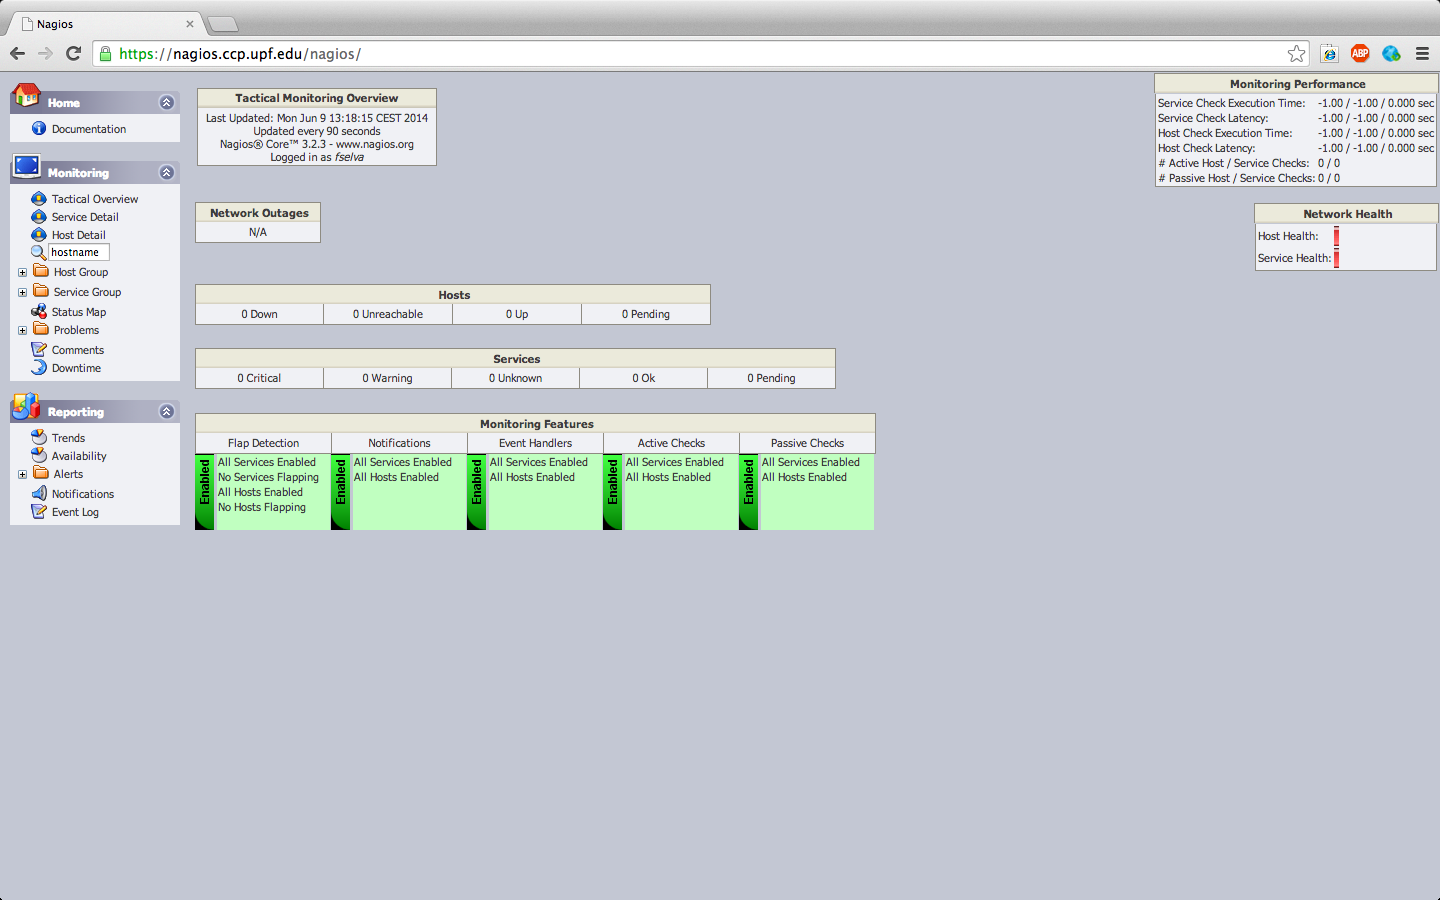
\includegraphics[scale=0.27]{./figures/Nagios.png}
              \rule{32em}{0.5pt}
          \caption[Nagios]{Nagios}
          \label{fig:nagios}
        \end{figure}

\subsection{ManageEngine OpManager}

OpManager, is a monitoring software for networks, servers and applications that helps the enterprises and service providers to manage its networks. It is developed by \textit{Manage Engine}, a brand of the ZOHO Corporation. Some of the features of this software are:
\begin{itemize}
\item Intelligent Alerts.
\item Automatic Workflows.
\item Quickly add of resources.
\item Automatic network discovery.
\item Network Mapping.
\end{itemize}

OpManager is used by companies and institutions such as at\&t, Siemens, NASA, Alcatel-Lucent or Time Warner \cite{opmanager}.


\chapter{SYSTEM COMPONENTS}
\label{Chapter3}

    \section{HARDWARE COMPONENTS}
        \subsection{Raspberry PI}
        Raspberry Pi [\ref{fig:raspberry}] is a computer with the size of a credit card, that can do the same things than a ordinary desktop computer. With this device it is possible to program, play games, browse the Internet, play High-definition videos and more. Raspberry Pi uses standard mouse and keyboard, and its interface is shown via HDMI cable. Raspberry Pi is developed by Raspberry Pi Foundation \cite{pi}.
        
        
        \begin{figure}[htbp]
          \centering
              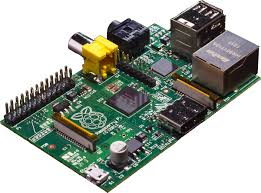
\includegraphics[scale=0.8]{./figures/raspberrypi.png}
              \rule{32em}{0.7pt}
          \caption[Raspberry PI]{Raspberry PI.}
          \label{fig:raspberry}
        \end{figure}
        
There are two models of Raspberry PI, Model A and Model B. For this project, it is used the Model B, because the model A has not Ethernet, a component needed for the correct operation of the Access program. Other differences are that model B has double USB connector and a 512MB Memory SDRAM.

    The components needed for the correct setup and operation of the Raspberry Pi Model B for this pilot are:
        \begin{itemize}
        \item \textbf{Micro-USB Power.} It is used to power the Raspberry PI. 
        \item \textbf{USB 2.0.} Needed to use USB devices, like the keyboard, or the mouse.
        \item \textbf{Ethernet.} Its function is to allow the Raspberry Pi connect to a Network.
        \item \textbf{HDMI connector}. It give the chance of display the Raspberry Pi interface on a Screen.
        \end{itemize}
        
    All those components, and more, like RCA Video connector or JACK Audio connector, are shown at figure \ref{fig:raspelem}.
        
        \begin{figure}[htbp]
          \centering
              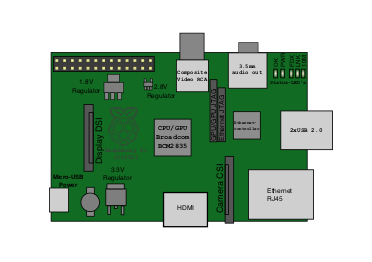
\includegraphics[scale=1]{./figures/Raspelem.png}
              \rule{32em}{0.7pt}
          \caption[Raspberry Pi Model B Components]{Raspberry Pi Model B Components}
          \label{fig:raspelem}
        \end{figure}
        
The operating system(OS) installed on the Raspberry Pi for this project is the Raspbian. It is based on Debian OS but it is optimized to work with Raspberry Pi hardware. This optimization consists in the pre-compiled software packages, that are included on this OS, making its installation easy, besides other features \cite{raspbian}.
        
        
        The Raspberry Pi used in this project has been configured to auto-start a process that will run a program to get and store information. As part of this, the Raspberry PI, must have installed Java Development Kit (JDK), to compile and execute Java projects. Projects like \textit{Access}, the program that runs the Raspberry PI. It is explained at section \ref{access}.
        
        
        \subsection{Server}
        A server, shown at figure \ref{fig:server}, is a computer that provides data to other computers using Internet. There are many types of servers. Each one uses different software to perform its purpose. The hardware used is not important. A computer can become a server with the appropriate software \cite{server}. 
        
        An example of these software is Apache HTTP. This software, used on web servers, is a open source code for the implementation of an HTTP server, that provides access to web applications using Internet connection \cite{apache}. 
        
        For this project it used a server from Universitat Pompeu Fabra, from Barcelona. It is a Debian machine, that has installed Apache HTTP and MongoDB, the database used to store the data. There is more information about MongoDB at section \ref{mongosection}.

        \begin{figure}[htbp]
          \centering
              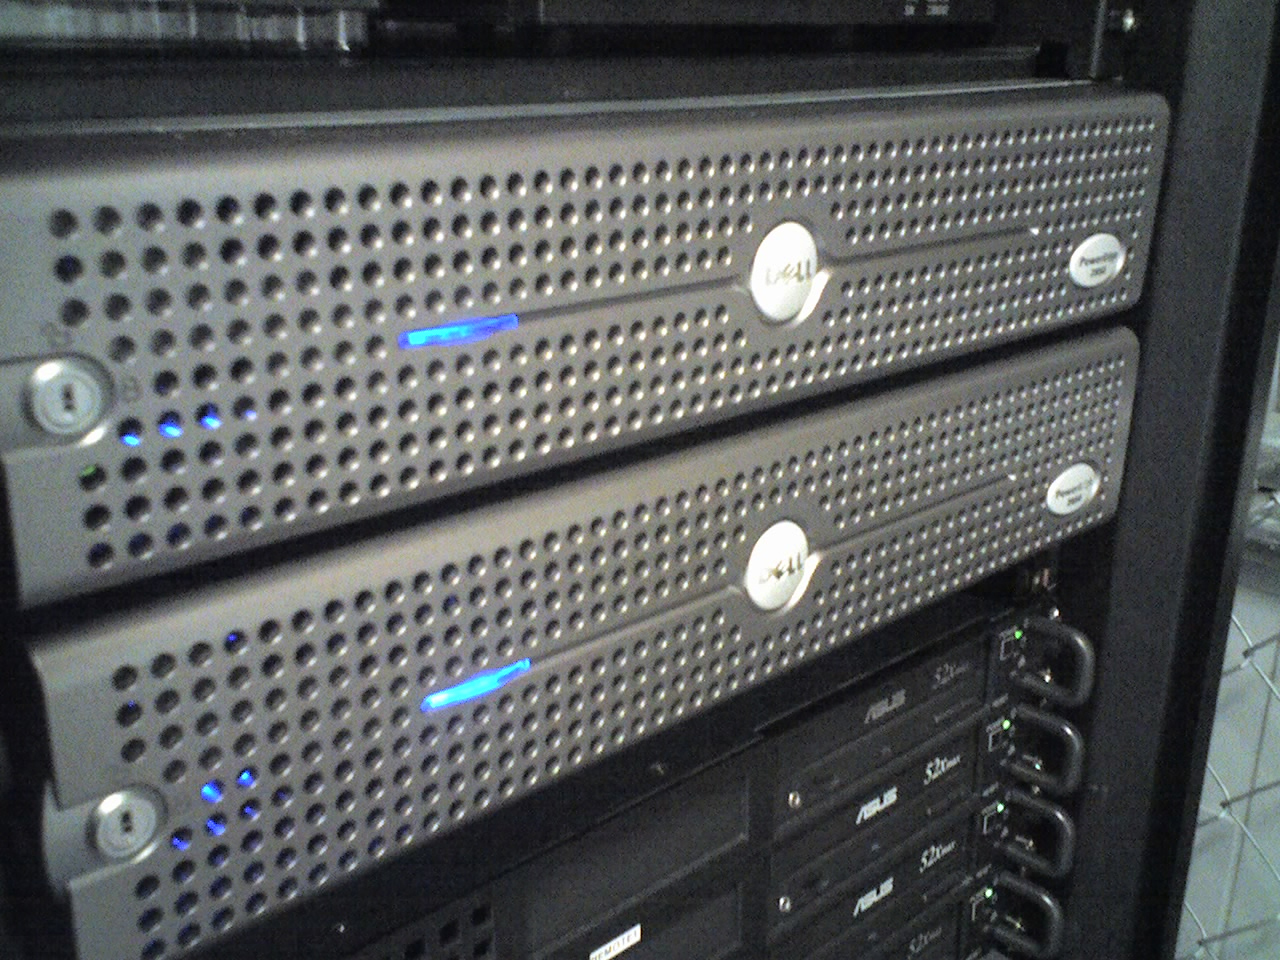
\includegraphics[scale=0.2]{./figures/Server.jpg}
              \rule{32em}{0.5pt}
          \caption[Server]{Dell Servers.}
          \label{fig:server}
        \end{figure}
        
        \subsection{Access Points}
        The Access Points (AP), figure \ref{fig:ap}, are devices which main goal is to connect other devices to a network. The access points have to be connected to a router, to provide them the network access. This network can be Internet network, or private networks. These devices will provide a secure access to network devices, like a server. 

        Often the access points and the router are integrated in one device, to which is added a switch for Ethernet cable connection. So, it is possible to access networks via wireless or cable with the same device \cite{ap}.
        
        
        %Para Poner debajo del texto deseado: \begin{figure}[H]
         \begin{figure}[htbp]
          \centering
              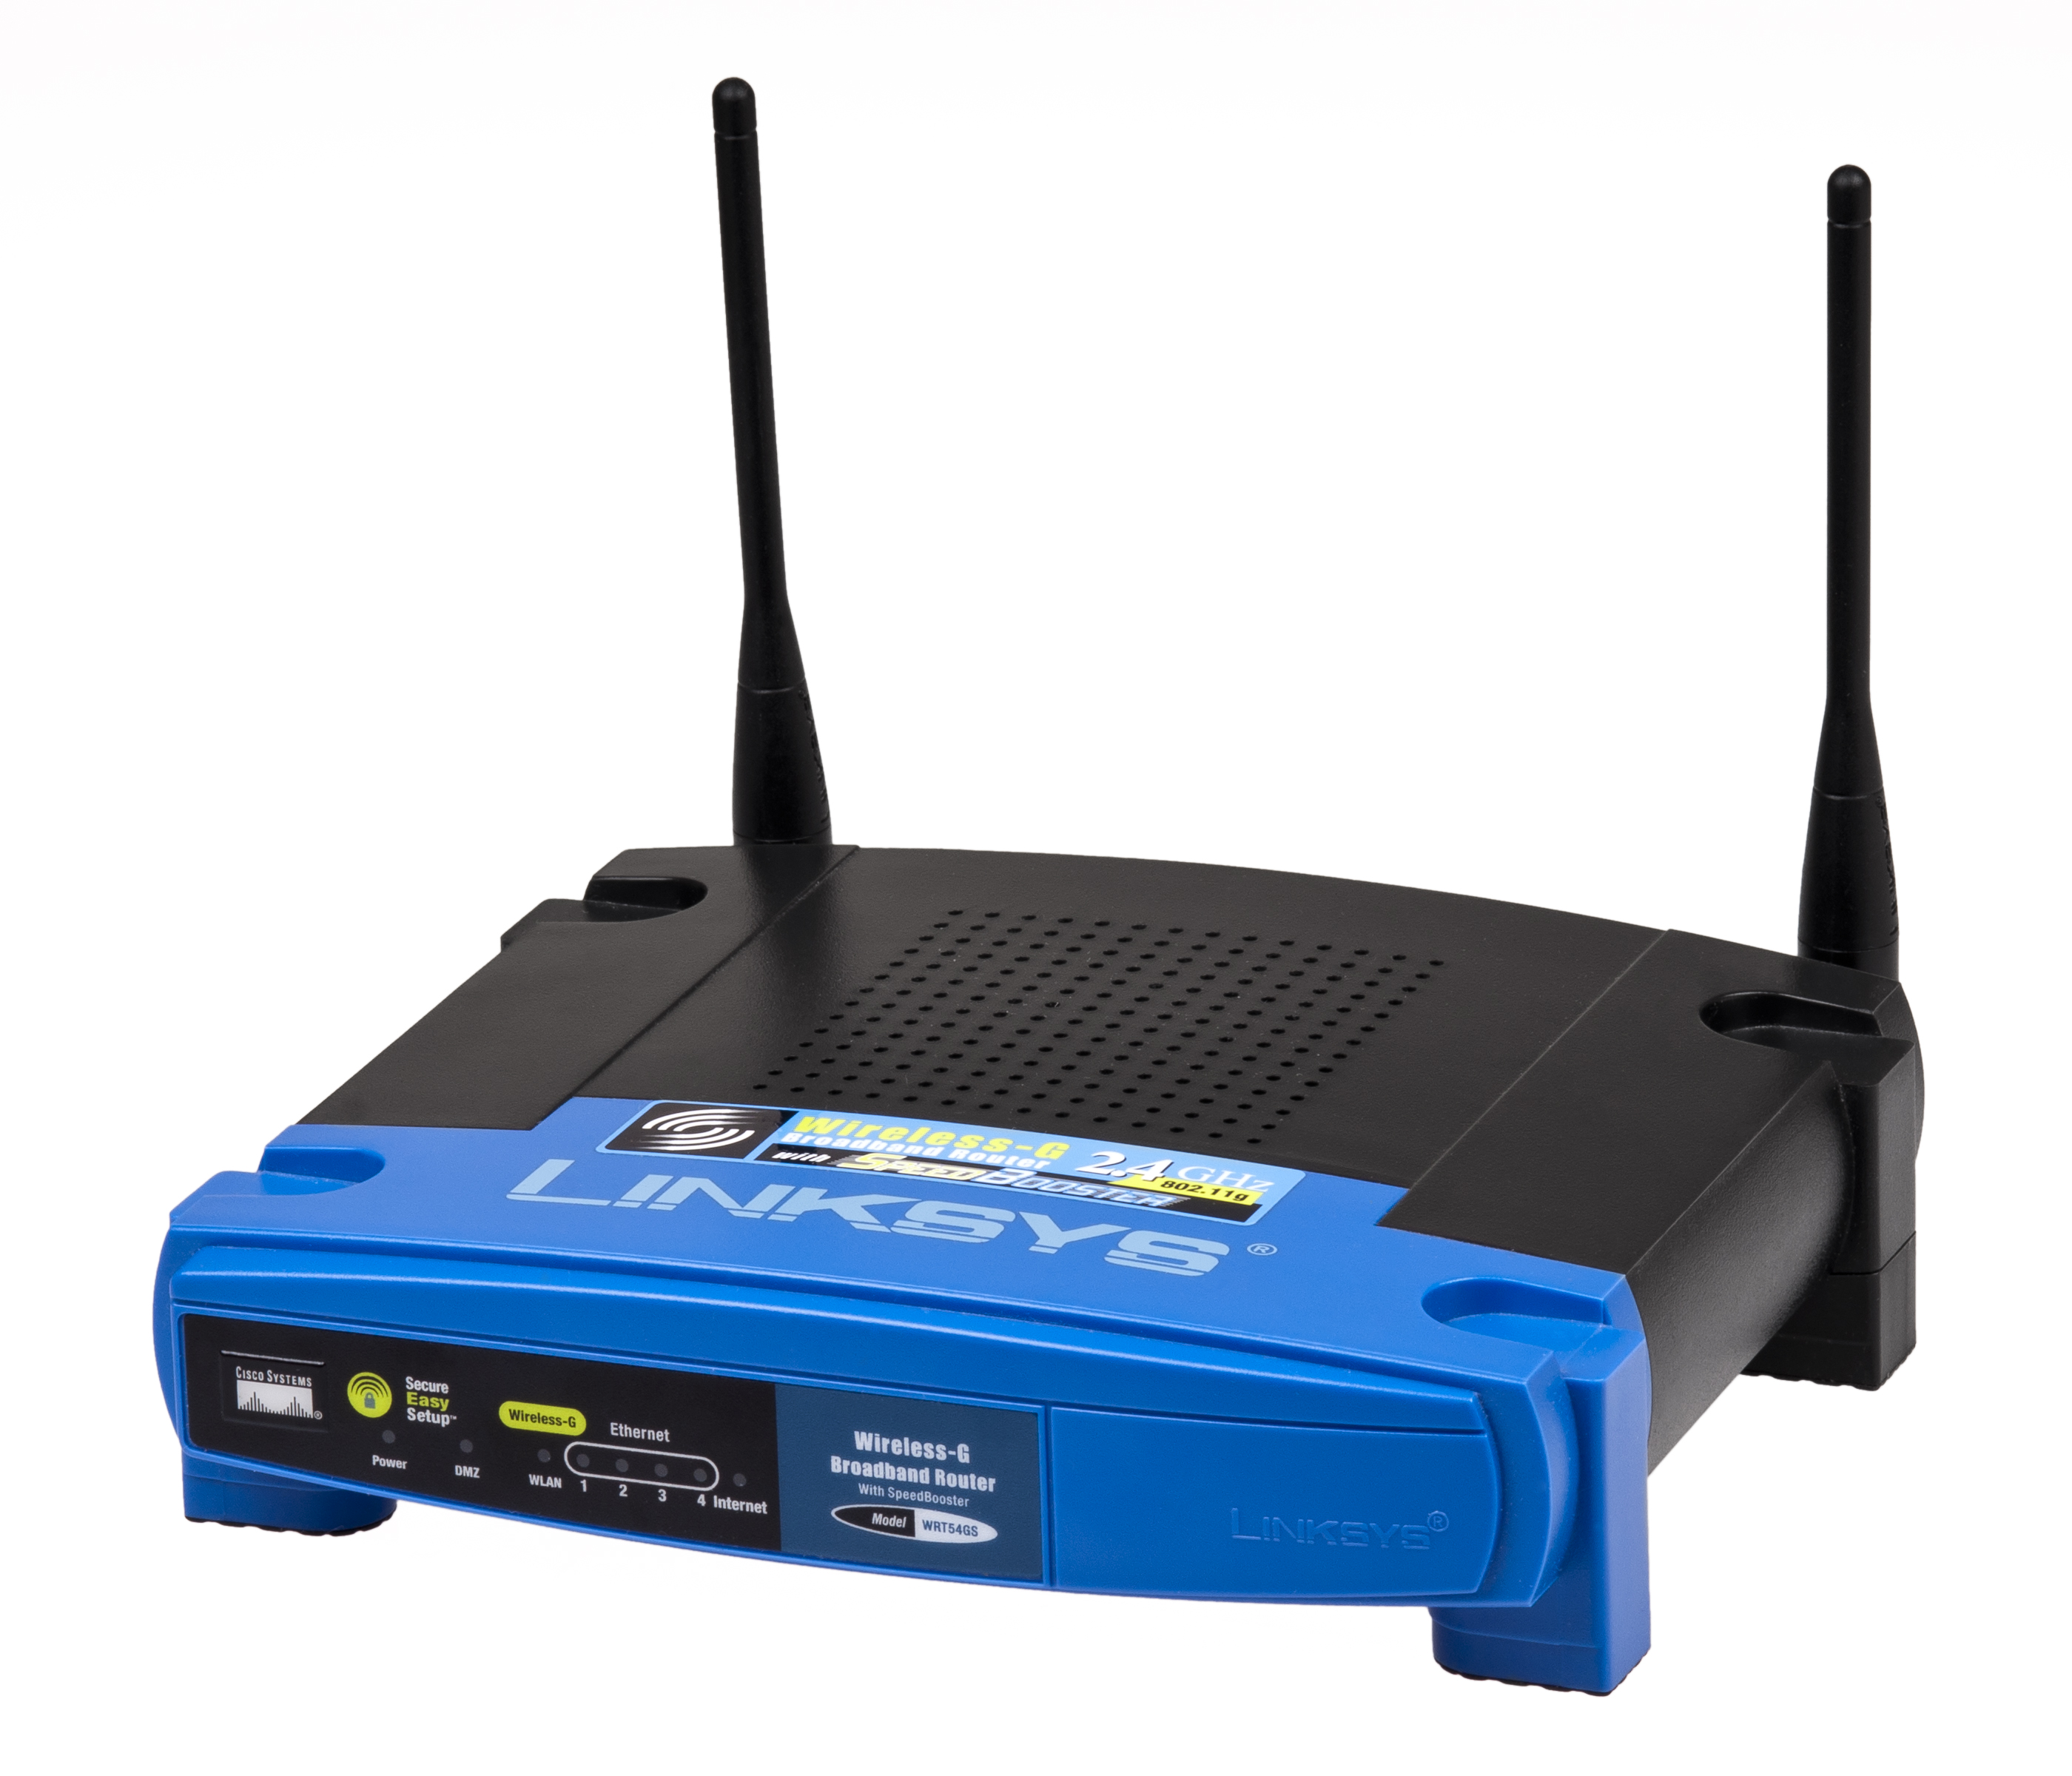
\includegraphics[scale=0.1]{./figures/Ap.png}
              \rule{32em}{0.5pt}
          \caption[Access Point]{Linksys WRT54Gt Access Point.}
          \label{fig:ap}
        \end{figure}
    
    \section{SOFTWARE COMPONENTS}
    
    At this chapter, it is explained the software elements used for the correct operation of the system. The code, and all the material of this project is public at \url{https://github.com/FerranSelva/Visual-Interface-Mashup-for-WiFi-and-Sensor-Networks.git}.
    
        \subsection{Access}
        \label{access}
        
      Access is a program made in Java, whose goal is to update the information about the status of the access points. This will be done by accessing these access points and obtaining all the information available. Information as the status, or the availability. Then the information is processed, and finally sent to the database. \\
        
        Java is a programming language developed in 1995 by Sun Microsystems, now acquired by Oracle Corporation. It is explained at section \ref{java}.\\
        
        To get the status of the access points, the program, pings the IP Address \footnote{IP Address: code that consist of four numbers separated with dots, needed to establish the connection between a device and Internet. Each one of this four numbers can can vary from 0 to 255 \cite{ipa}.} of the access points. If this ping is successful, it means that the access point is working correctly. Then with this status, and using device time, the information is processed to get the availability, the uptime, downtime and since when the access point is on or off. 
        
        Once this information is processed, it is sent to the database located at a server. This transfer of information is done using a web service called by the program, that will access and modify the database locally. The web service is described at section \ref{web service}.
        
If the program is stopped, or an access point is not working, the Access program, using a method of the web service will send an email to the network manager, with a description of the problem. This reporting will help the manager resolving issues easily.
        
        Each class of this program has a function, and some of them have the same name than the web server method that uses. The section \ref{classes} discuses about these classes.\\
        
The Access program is located at the Raspberry PI, and it is ran when the device is started, this program will not stop until the user give this order. To work properly, the Raspberry Pi should be located at the same network of the access points to have access via ICMP. While ICMP is used, usually, to report an error in the datagram processing, in this system, it is used to know the status of the hotspots.\\

            It is described ICMP at section \ref{icmp}.

            \paragraph{Java}
            \label{java}\\
            Java is a programming language, used to develop all type of programmes. Programmes like games, mobile application, enterprise software and more. 
            Java has been tested, improved and extended by Java developers. The results of this actions are that Java is fast and secure \cite{Java}. 
            
            Java allows developers to:
            \begin{itemize}
            \item Write software on one platform and run it on other platforms.
            \item Create web browser runnable programs that can  access web services.
            \item Develop server-side applications.
            \item Combine applications or services.
            \item Write applications for multiple devices, like mobile phones, microcontrollers and others.
\end{itemize}
            
           For this project, it is used classes such as \emph{HttpURLConnection}, \emph{Runtime} or \emph{BufferedReader}. The first, \emph{HttpURLConnection}, is used to connect the program with the web service. \emph{Runtime} is used to run terminal commands. The command to be run is a ping to an access point. To get the response of the ping, it is used the class \emph{BufferedReader}, that gets the response from the web service or terminal. 
             
            
            \paragraph{ICMP}
            \label{icmp}\\
            Internet Control Message Protocol(ICMP) is a Protocol used to control purposes between connected devices. This control is done via messages, that give feedback of the problems that are happening in the network \cite{icmp}.\\
            
            ICMP messages structure is shown at the figure \ref{fig:ICMP}.
            
            
        \begin{figure}[htbp]
          \centering
              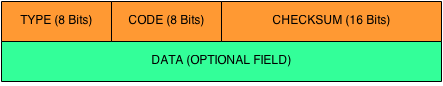
\includegraphics[scale=0.7]{./figures/ICMP.png}
              \rule{32em}{0.5pt}
          \caption[ICMP Messages Structure]{ICMP Messages Structure}
          \label{fig:ICMP}
        \end{figure}

        \\
       
       For this project, the main goal of ICMP is to get the availability of the access points of a network. Using the ping response at the terminal, the program Access determines if the access point is UP or DOWN.\\
        
        It is shown the Raspberry Pi running the Access program, at the figure \ref{fig:Rasprun}
        
        \begin{figure}[htbp]
          \centering
              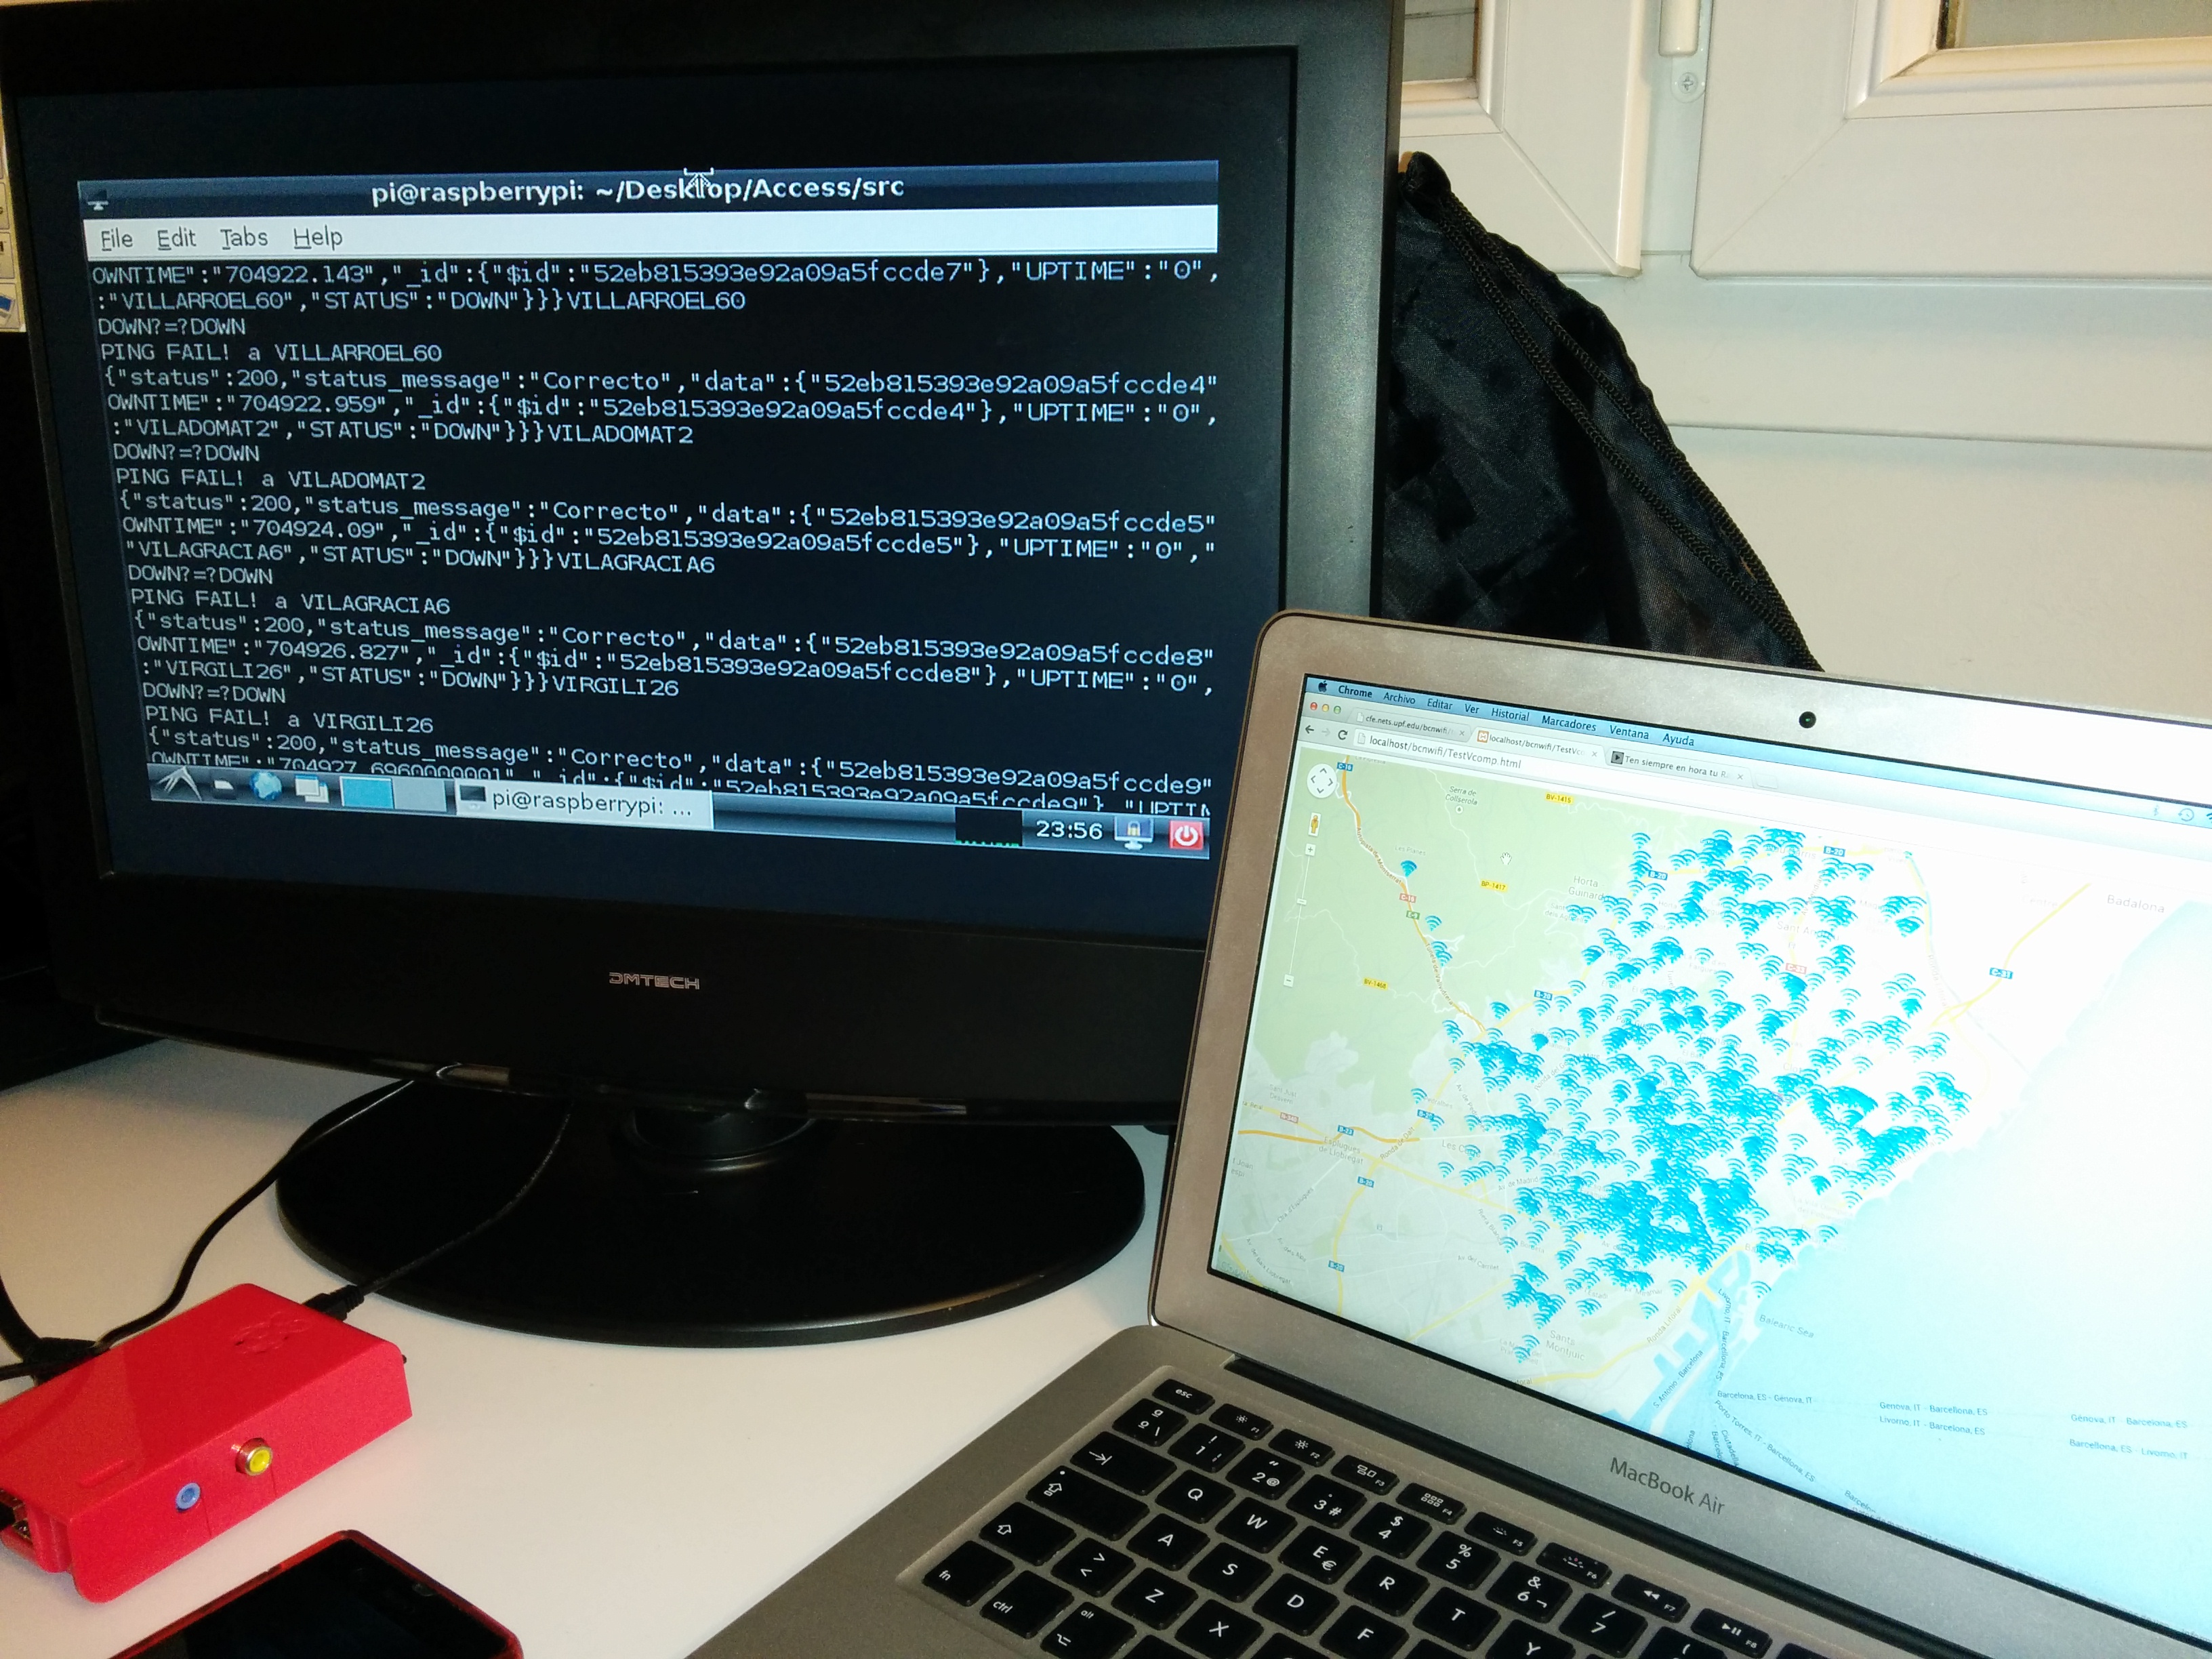
\includegraphics[scale=0.12]{./figures/RaspRun.jpg}
              \rule{32em}{0.5pt}
          \caption[Access program running on a Raspberry PI]{Access program running on a Raspberry PI}
          \label{fig:Rasprun}
        \end{figure}

           
        
            \subsubsection{Classes}
            \label{classes}
                \paragraph{ConnectionMongo.java}
                
                ConnectionMongo is the main class of the program. This will call other classes when needed. This class will begin, getting the ID and the corresponding IP, of all nodes of the network. This will be done using the methods \textit{FindID()} and \textit{FindIP()} from the class getData, described at section \ref{getData.java}. Then, it will run a sequence until the process stop or the Raspberry Pi powers off. This sequence will start doing a ping to each node using method \textit{doPing()} of the Ping class. Next step is to update Resume collection from the database, using updateResume, getlastupdate, and postResume classes. The fields ``STATUS", ``SINCE", ``TOTALTIME", ``UPTIME", ``DOWNTIME" and ``AVAILABILITY" will be updated. Then the program will insert to Data collection all the information collected for later use.\\
            
                \paragraph{getData.java}
                \label{getData.java}
                 
                GetData is the class used to get the ID and the IP of the access points. This class has three methods. The first one, \textit{getresult()}, calls a web service, to get all the information stored on the database about the nodes. The second one, \textit{FindIP()}, will return a vector with all IPs. And the third one, \textit{FindID()}, will return a vector with the ID of all nodes.\\

                \paragraph{getUTDT.java}
                
                The class getUTDT has the objective of get the Uptime, the Downtime and the status of a specific node. This class can call three methods. The method \textit{getuptime()} will get the uptime of a specific node using its ID. The second one, \textit{getdowntime}, will get the downtime of a node. And the last method, \textit{getstate()}, will return the status of a node.\\
                
                \paragraph{getlastupdate.java}
                
                Getlastupdate aims to get the last update values. This is needed to process the information, and calculate values such as availability, totaltime, or others. The first method included in this class, is \textit{getresult()}. This method uses the web service to get the information about last update of a node. The second one is \textit{getlastTimestamp()} that will get the last Timestamp from a node. And the last, \textit{isDataempty()}, checks if the database is empty or not.\\
                \\

                \paragraph{Ping.java}
                
                Class Ping is used to do a a ping to the access points. This class has a unique method called \textit{doPing()}, that will use ICMP protocol to do a ping to a specific node. The method \textit{doPing} is a boolean that will return true or false, depending on the response received of the ping.\\
                
                \paragraph{postData.java}
                
                The class postData is used to insert information about the access points to the Data collection. This class calls a method \textit{insertdata()}, that will use a web service to insert to the collection Data a document with the ID, the status, and the timestamp of a hotspot. \\
                
                \paragraph{postResume.java}
                This class objective is to update the information of an access point on the Resume collection. This class calls two methods, \textit{modifystate()}, that will update the status of an access point. And \textit{modifytime()} is used to modify the other values related to the time, this values are totaltime, uptime, downtime and availability. The class \emph{postResume} will be called in the class updateResume.\\
                
                \paragraph{updateResume.java}
                This class aims to process the information gotten, and update the Resume collection with the results. The class updateResume has a unique method \textit{update()} that will use postResume class to update the database.
                
                If an access point is DOWN, this class will use Sendmail class to send a mail with the goal of notify the network manager of this event.\\
                
                 \paragraph{Sendmail.java}
                 The main objective of the Sendmail class is to send a post request to the web service who will send an email to an specific address.
                 
                 This class calls a method \textit{send()}, it is used to notify the manager of the network when the program is stopped, or when an access point is down.
                 When it is notifying the program stop, the program sends the cause of this stop using \textit{Java Exceptions}.
                 When it is notifying the down status of an access point it sends the ID of the node that is not working properly.

                 The report of a DOWN status of an access point is done the first time that a hotspot is DOWN. That means that if in the last iteration, the status of an access points was DOWN, and now is again DOWN, the program will not send a mail, because it keeps DOWN, at least, since the last iteration.
                So, to receive another email about the DOWN status of these access points, it is needed the change from UP to DOWN of the status of a hotspot.
                 
        
            \subsubsection{Flowchart}
            
            The flowchart that describes the behaviour of the Access program is shown at the figure \ref{fig:accessp}. 
            % Afegir enviar mail si el programa es para!
            \begin{figure}[htbp]
              \centering
                  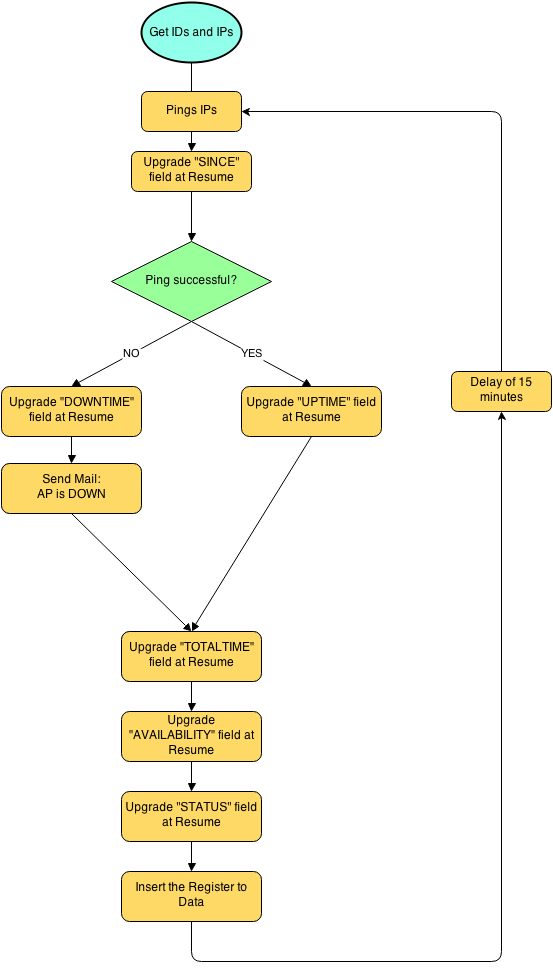
\includegraphics[scale=0.5]{./figures/Flowchart.png}
                  \rule{32em}{0.5pt}
              \caption[Access Program FlowChart]{FlowChart}
              \label{fig:accessp}
            \end{figure}
        
            \subsubsection{Class Diagram}
            
            The Class diagram of the Access program is shown at the figure \ref{fig:classdiagram}
            
             \begin{figure}[htbp]
              \centering
                  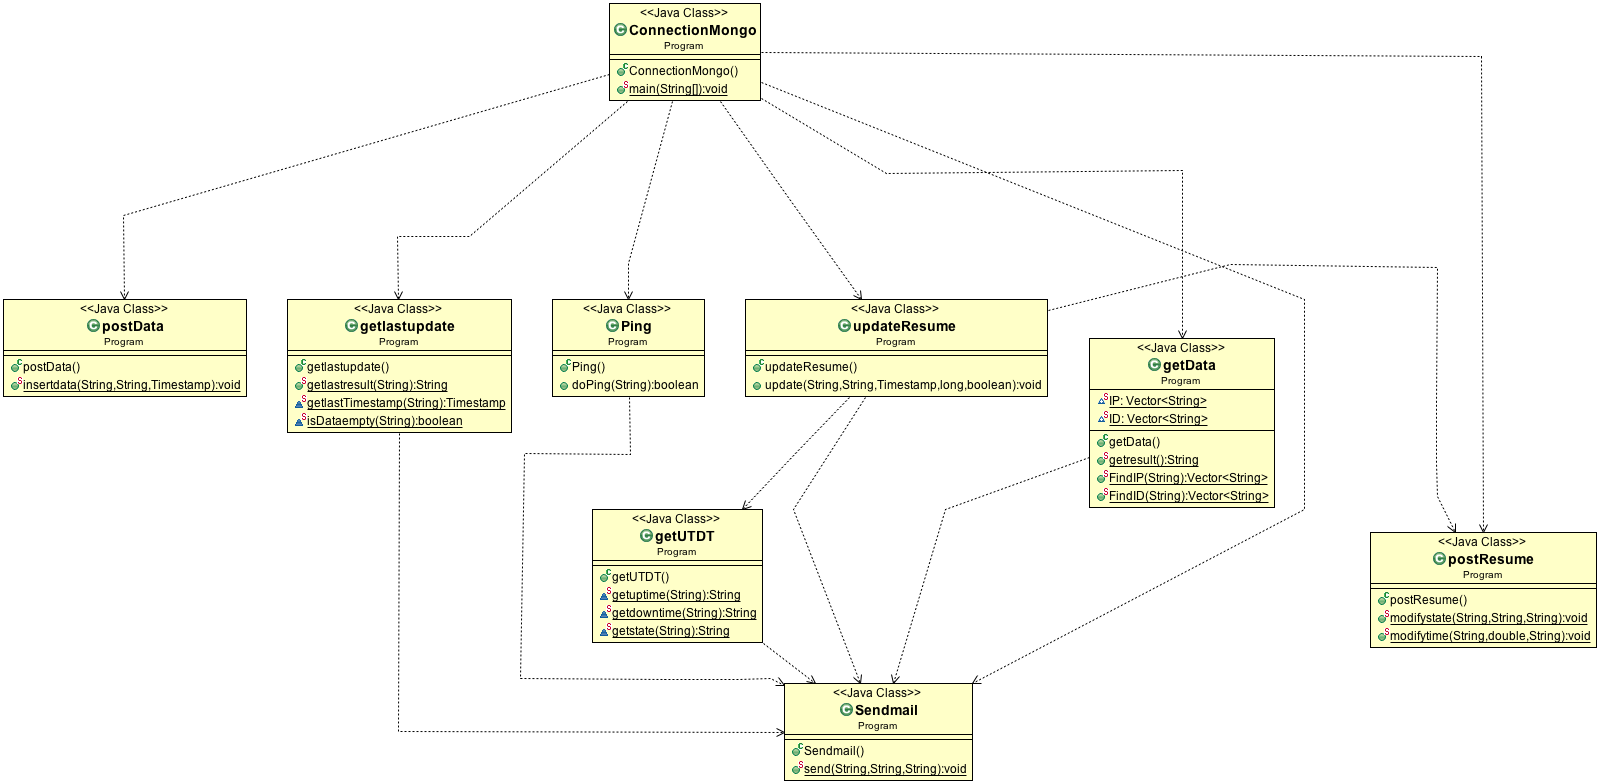
\includegraphics[scale=0.35,angle=90]{./figures/Classes.png}
                  \rule{32em}{0.5pt}
              \caption[Access Program Class Diagram]{Access Program Class Diagram}
              \label{fig:classdiagram}
            \end{figure}
            
        \subsection{Web Application}
        
        
        The web application, is the tool used to display the information about the access points of a network to the managers of the network or its users. The information is gotten from the collection Resume of the database, located at the server.
        
            \subsubsection{Components}
            The web application needs three files, each one written in different language. These program languages are HTML, Javascript and PHP.
The files that compose this web application are:
                \paragraph{index.html}
                Index.html is the file written in Hyper-Text Markup Language (HTML). HTML is a markup language used to create hypertext documents. These documents are platform independent. This means that are portable from one platform to another platform. This language is used by the World-Wide Web (WWW) global information initiative since 1990 \cite{html}.
                
In this case, \emph{index.html} sets a Google maps map and calls the function.js javascript, to set values of the map.

                \paragraph{function.js}
                The file function.js, is a javascript file. Javascript, designed by Sun Microsystems, is based on the Java syntax. It is a scripting language, what means that can be used to write stand-alone programs \cite{javascript}.
                
       Function.js, for begin, will call the getinfo.php file to get the data from the MongoDB database. Next step, is to parse the data obtained from the database. Finally, it will use the parsed data to add the information to the google maps map using infowindows.
       
       These infowindows are pop up windows that display information on a specific location on the map. In this case each infowindow will contain the information of an access point, and will be positioned at its location \cite{infowindow}.
                
                \paragraph{getinfo.php}
                Getinfo.php is written in PHP. This file will get the database values and return these to the javascript to be parsed and displayed. PHP is explained at the following paragraph \ref{php}.\\
                
                \paragraph{PHP}\\
                \label{php}
                Hypertext Preprocessor (PHP), is a HTML-embedded Web scripting language. This means that HTML files can contain PHP code. This programming language is used for the web development. It main purposes are:
                \begin{itemize}
                \item{Scripting on the server-side.}
                \item{Command line scripting.}
                \item{Writing desktop applications (Not used very usually).}
                \end{itemize}\\
                
                PHP is read/ran at the server and the output has HTML format. So, this output will be readable by the browsers. PHP is a good option to access databases, because the php code is not shown on the page \cite{php}.
                
                In this project, PHP is used by the web application, to get the information that will be displayed in the map.
                 
                Also PHP makes possible the information exchange between the Raspberry Pi and the Server. This is done using a web service composed by the PHP files. This PHP files use a Mongodb module to access the information stored.\\


It is shown the web application that shows the status of the access points from \textit{guifi.net}\footnote{\textit{guifi.net} is an open and free network, build for all who want to join. The user will provide his connection, this will extend the network, and consequently the user will get more connectivity to other nodes of this network \cite{guifinet}.} network at the figure \ref{fig:wapp}.

        \begin{figure}[htbp]
          \centering
              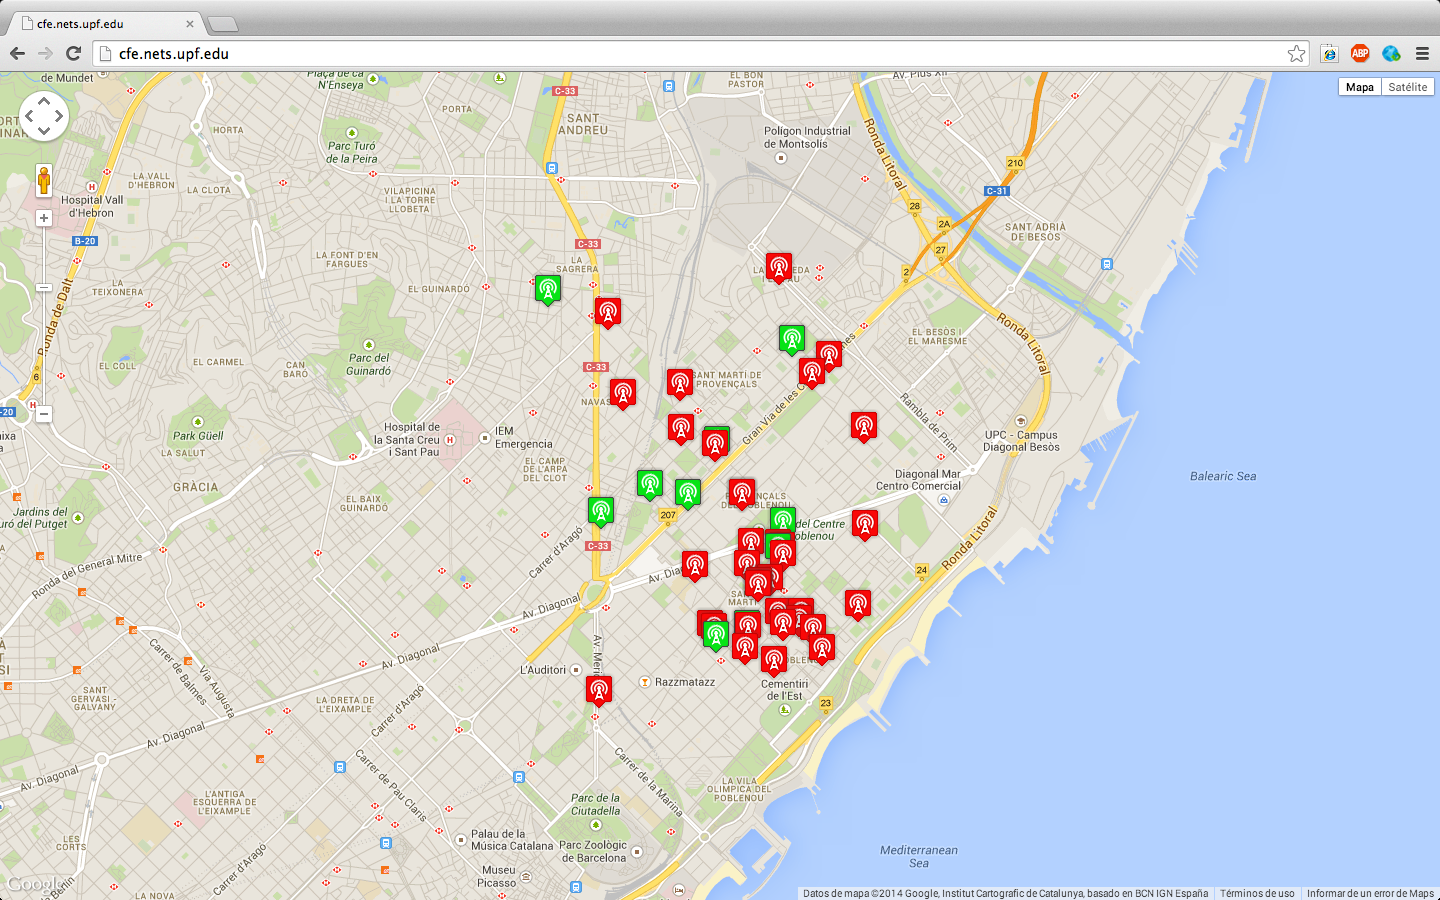
\includegraphics[scale=0.3]{./figures/WebApplication.png}
              \rule{32em}{0.5pt}
          \caption[Web Application]{Web Application}
          \label{fig:wapp}
        \end{figure}
        
        
        \subsection{MongoDB Database}
        \label{mongosection}
        MongoDB[\ref{fig:MongoDB}] is a an open-source NoSQL database that works with BSON objects, similar to JSON objects. The main features of this kind of database are the high scalability, performance and availability \cite{mongo}.
        
        \begin{figure}[H]
          \centering
              
\includegraphics[scale=0.2]{./figures/mdblogo.png}
              \rule{32em}{0.5pt}
          \caption[MongoDB Logo]{MongoDB}
          \label{fig:MongoDB}
        \end{figure}
        
        
        MongoDB main features are:
        \begin{itemize}
        \item BSON Document Data Model.
        \item Idiomatic Drivers. There are MongoDB drivers for the main program languages. Languages such as Java, Ruby, PHP, JavaScript or others.
        \item Horizontal Scalability.
        \item High Availability.
        \item In-Memory Performance.
        \end{itemize}
        
        MongoDB capabilities, structure and applications are shown at the figure \ref{fig:MongoDB Stack}. 
        
        \begin{figure}[H]
          \centering
              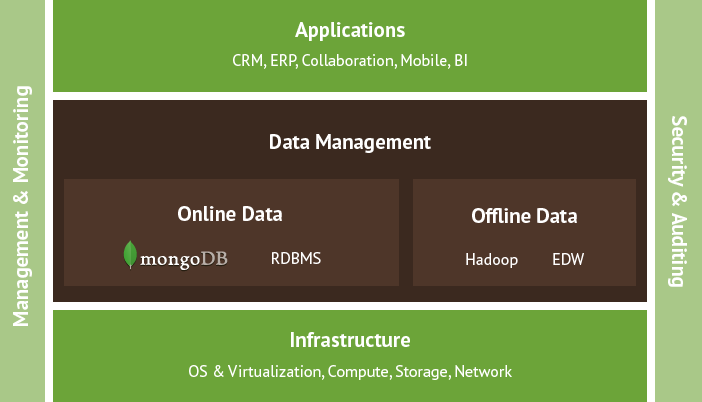
\includegraphics[scale=0.5]{./figures/mfeatures.png}
              \rule{32em}{0.5pt}
          \caption[MongoDB Stack]{MongoDB Stack}
          \label{fig:MongoDB Stack}
        \end{figure}
        
            \subsubsection{Why MongoDB?}
            
            For this project, the database used is MongoDB. The decision of use MongoDB, a NoSQL database, instead of SQL-based databases is explained at the following paragraphs.
            
           NoSQL databases were developed with the objective of solve the limitations of the SQL-based Databases. The main limitations to be solved were the scalability, a important feature for this project, the replication, and the unstructured data storage.
           
           The result of this development is that NoSQL databases have better performance and are more scalable than SQL ones. In addition, NoSQL databases have better results when talking in terms of holding a large volume of data, quick iterations, object-oriented programming, and scalability \cite{nosql}.

        Its cost is cheaper than SQL-based ones. All NoSQL databases are open-source, while SQL ones, can be open-source or closed source. Another benefit is that NoSQL databases are dynamic while SQL ones are fixed.
        
        All those features, suggest that the best choice is NoSQL Databases, and specifically MongoDB because it is simple to use and has a good performance \cite{nosql}.

            \subsubsection{Operation}
            \paragraph{BSON}\\
            MongoDB uses Binary JSON(BSON) documents, to store the data. This documents are very similar to JSON objects. A benefit of BSON is that these type of documents have more data types. Types like Date. A second benefit is that JSON and BSON are flexible. The con is the efficiency because BSON messages have an overhead produced by the field names \cite{bson}.\\
            
            The main features of BSON are:
            \begin{itemize}
            \item Lightweight.
            \item Traversable.
            \item Efficient. Related to fast encoding/decoding.
            \end{itemize}
            
            \paragraph{Structure}\\
            
            MongoDB has three levels in its structure. The top level is the Databases. Databases are biggest elements that contains collections. The collections are the middle elements that contain the mass of documents. The documents are the smallest and primary element to store the data.
            
        \begin{figure}[htbp]
          \centering
              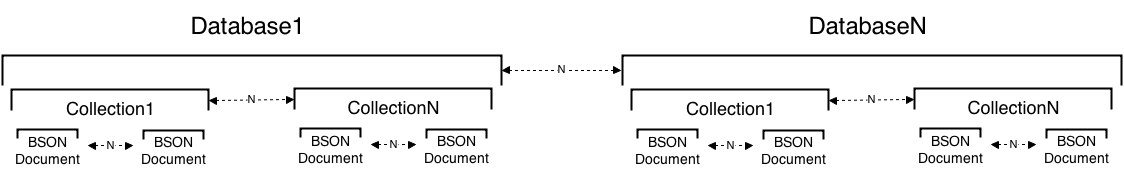
\includegraphics[scale=0.35,angle=0]{./figures/mstr.png}
              \rule{32em}{0.5pt}
            \caption[MongoDB Structure]{MongoDB Structure}
            \label{fig:mstruc}
        \end{figure}
            
            \paragraph{Commands}\\
            The commands that are needed for the correct operation of the system are \cite{mongocmd}:
            \begin{itemize}
            \item \textbf{Find}
            
            find() command is used to obtain the documents from a collection. These documents can be obtained with different options, like obtain by a specific field value, sort documents, and other.
            The structure of this command is: \\
            
            \centerline{\textbf{db.collection.find(\textless criteria\textgreater, \textless projection\textgreater)}}\\
            
            where \textit{collection} is the name of the collection from where the documents will be obtained. \textit{Criteria} and \textit{projection} are optional fields. The first one, \textit{Criteria}, is a field used to find documents that follow a specific conditions. It is possible to set ``equal" condition, ``greater" condition, and others. The second one, \textit{projection}, define the fields of the documents to be returned.
            
            \item \textbf{Update}
            
            This order will modify existing documents of a collection. The modification can be done by one or multiple documents. The structure of a update command is: \\
            
            \centerline{\textbf{db.collection.update(query, update, options)}}\\
            \textit{query} and \textit{update}, are mandatory fields. These fields are used to define a selection criteria, and for define the modifications to be done, respectively. \textit{Options} field is used to add some features like ``upsert" or ``multi".
            
            \item \textbf{Insert}
            
            This function adds new documents to a collection. This command follow the next syntax: \\
                
            \centerline{\textbf{db.collection.insert(\textless document\textgreater)}}\\
            where the \textit{document} is the document or array of documents to add to the collection.
                
            \item \textbf{Remove}
            
            It removes documents of a collection. Its syntax is:\\
            
            \centerline{\textbf{db.collection.remove(query, options)}}\\
            
            \textit{query} is a mandatory field, witch specify the deleting criteria. \textit{Options} field is to add features like ``justOne" or ``writeConcern".
            
            
            \end{itemize}

            \subsubsection{Collections}
            
            For the correct operation of the system, there are needed two collections. These collections are described next:
            \paragraph{Resume}
            
            Collection Resume stores all Access Point information using a document per Access Point. The information included in these documents, for each Access Point is: 
            \begin{itemize}
            \item ID.
            \item IP.
            \item Latitude.
            \item Longitude.
            \item Status.
            \item Since (This field save the last time when the status changed).
            \item Totaltime.
            \item Uptime.
            \item Downtime.
            \item Availability.
            \end{itemize}
            
            The last six fields, status, since, totaltime, uptime, downtime and availability, will be modified, updating these values for the current ones. This current ones will be obtained and modified on this collection by the Access program on the Raspberry Pi.
            
            \paragraph{Data}
            
            This collection stores the register of the status of the Access Points. This register consists on documents with three fields, \textit{ID}, \textit{STATUS} and \textit{Timestamp}. 
            The information stored will be processed using Access program, and with the result, the documents on Resume collection will be updated.
            This collection can be very useful for the implementation of future features.
        
        \subsection{Web service}
        \label{web service}
        The web service, implemented for this system is a RESTful web service, composed by six PHP files. Its main objective is to be the way of communication that will be used to connect the Raspberry Pi with MongoDB Database at the server. 
        
        This web service will use mongo-php-driver. With this driver, PHP is able to use classes and functions that, specifically, get, modify, create or set up databases and its values of MongoDB. There are four types of methods, GET, POST, PUT and DELETE. For this web service, the methods used are:
            \subsubsection{GET Methods}
            GET Methods are used to retrieve for specific data, in this case, from the MongoDB database. The get methods of this webservice are:
                \paragraph{getData.php}
                This method retrieves the data needed by the Access program to ping the access points. These data will be the ID and the IP of each node of the Network. The data will be obtained from the Resume collection. An example of the getData response is shown at the figure \ref{fig:phpre}.
                
        \begin{figure}[H]
          \centering
              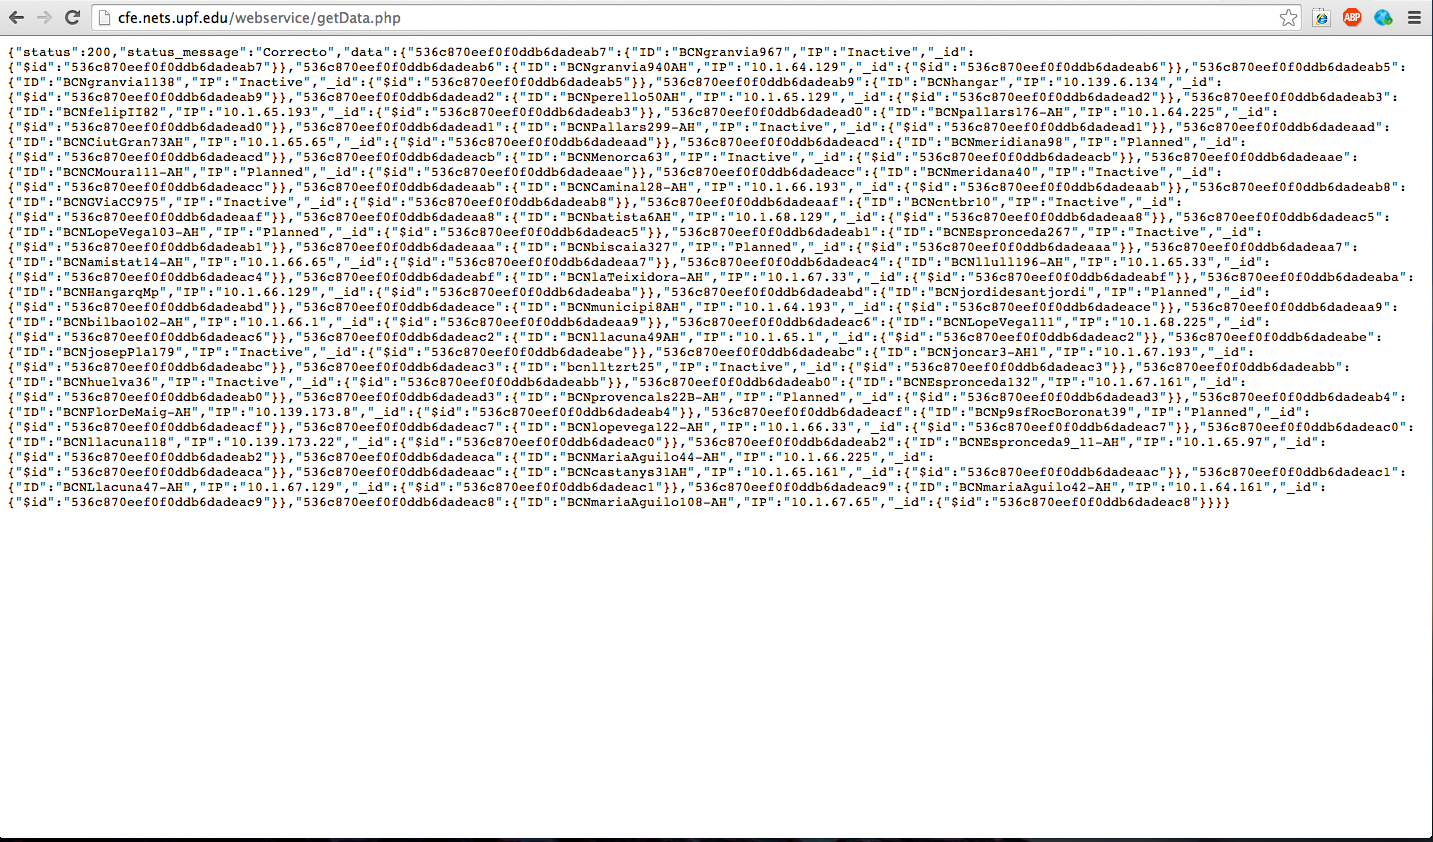
\includegraphics[scale=0.3,angle=0]{./figures/phpresponse.png}
              \rule{32em}{0.5pt}
            \caption[Response of getData Method]{Response of getData Method}
            \label{fig:phpre}
        \end{figure}
                
                \paragraph{getUTDT.php}
                The method \textit{getUTDT} gets the Uptime and Downtime fields of an specific node from the Resume collection. This information is needed by the Access program to process and calculate the new values for the fields Totaltime, Availability, Uptime and Downtime.
                
                This method requires the parameter \textit{id}, referred to the ID of the node to be updated.
                
                \paragraph{getlast.php}
                \textit{Getlast} is a method that retrieves the last register of the Data collection for a specific node. This register refers to the last update of the Access program. This information is required to update the SINCE field of the Resume collection and to know how much time has passed since the last update.
                
                The parameter \textit{id} is needed to select the node, whose information will be obtained.
            
            \subsubsection{POST Methods}
            POST Methods, similar to PUT, add or update new data to the database. The POST methods for this system are:
            
                \paragraph{postResume.php}
                
                The method \textit{postResume}, called by the Access program, is used to update the values of the fields contained to the Resume collection. The fields to be modified will be: 
                \begin{itemize}
                \item Status.
                \item Since
                \item Totaltime.
                \item Uptime.
                \item Downtime.
                \item Availability.
                \end{itemize}
                
                The method, require three parameters, the \textit{field} to be updated, the new \textit{value} of the field, and the \textit{id} of the node whose field will be modified.\\
                
                
                \paragraph{postData.php}
                This method is used by the Access program to add new documents to the Data collection. The insertion of these documents will happen each time that Access program pings to a hotspot, and the result of these pings is stored in those documents. These documents, to be inserted, should have the fields ID, STATUS and TimeStamp. 
                
                So the parameters needed for this method are \textit{id}, \textit{status} and \textit{timestamp}.\\
                
                \paragraph{notify.php}
                This method is used to send an email, when the Access program calls this method using a POST request. The mails sent are used to notify the manager of the network that something is going wrong. This bad operation can be produced because the Access program has been stopped or a hotspot is not working properly for some reason.
                
                The parameters needed to the correct operation of this method are \textit{id}, \textit{type} and \textit{e}. This \textit{e} is the exception that is returned by the Access program, when it has been stopped. This parameter will help to locate the error and repair it.
                
 \chapter{SYSTEM OPERATION}
\label{Chapter4}

The structure of the system is illustrated at figure \ref{fig:arq}. The following paragraphs will contain the explanation of the operation of the elements illustrated, and its importance inside the system.
        
        The system can be divided into two sections. A section that gets and stores the information about the hotspots. And another section that processes the information, and displays it with a format that everyone could understand.
                
        The elements of the first section mentioned are: 
        \begin{itemize}
            \item Raspberry PI.
            \item Server.
            \item Hotspots. 
        \end{itemize}
        
        The operation of this section will begin with the implementation of a Raspberry Pi into the same network that the access points to be monitored. Once the Raspberry Pi is booted, it begin, automatically, a process that executes the Access program, explained at section \ref{access}. This program will try to ping access points of the network. The IPs to be pinged, have to be gotten from the database located at server using getData method. When the pings are done, the information about this access points is processed. Then the Raspberry PI, using the program, must access to a web service, located at the server, to store the information.
        
       % Falta Afegir Text: "Servidor"
       %eliminar IMI (en el cloud)
       % indicar que es coloqui en vertical.
        
        \begin{figure}[htbp]
          \centering
              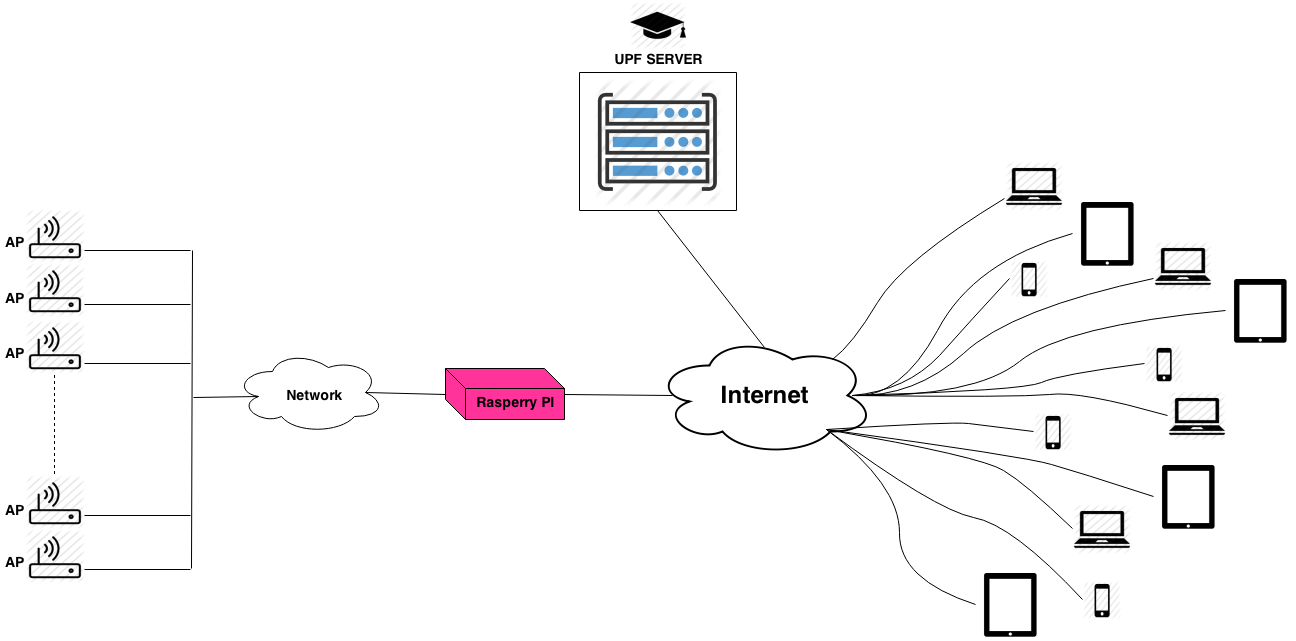
\includegraphics[scale=0.42,angle=90]{./figures/arq.png}
              \rule{32em}{0.5pt}
            \caption[System Diagram]{System Diagram}
            \label{fig:arq}
        \end{figure}
        
        The server will receive and store the information about the access points. The storage of this information will be done by the MongoDB database, and the communication between Access program and the database is done using a web service.\\
        
        The other section, use the following elements:
          \begin{itemize}
            \item Server.
            \item Users Devices.
        \end{itemize}
        
        This section main goal is to display, using a web application, the information once this has been gotten and processed with a simple format to let everyone understand it. The web application is located at the server, and using Apache HTTP, will serve a web application, at the domain \url{http://cfe.nets.upf.edu/}. This web application will show, at the location of the access points, the information stored at the database. Or, what is the same, the information gathered at the previous section.\\
        
        The citizen, only has to open the browser at the domain \url{http://cfe.nets.upf.edu/} to check the status of the access points of the network being monitored.
        
        To change the network to be monitored, it is needed to add the  access points information to the database before starting the Raspberry Pi, and, in consequence, the Access program. The information needed is the IP and the ID of the nodes to be monitored.
        
        \begin{figure}[htbp]
          \centering
              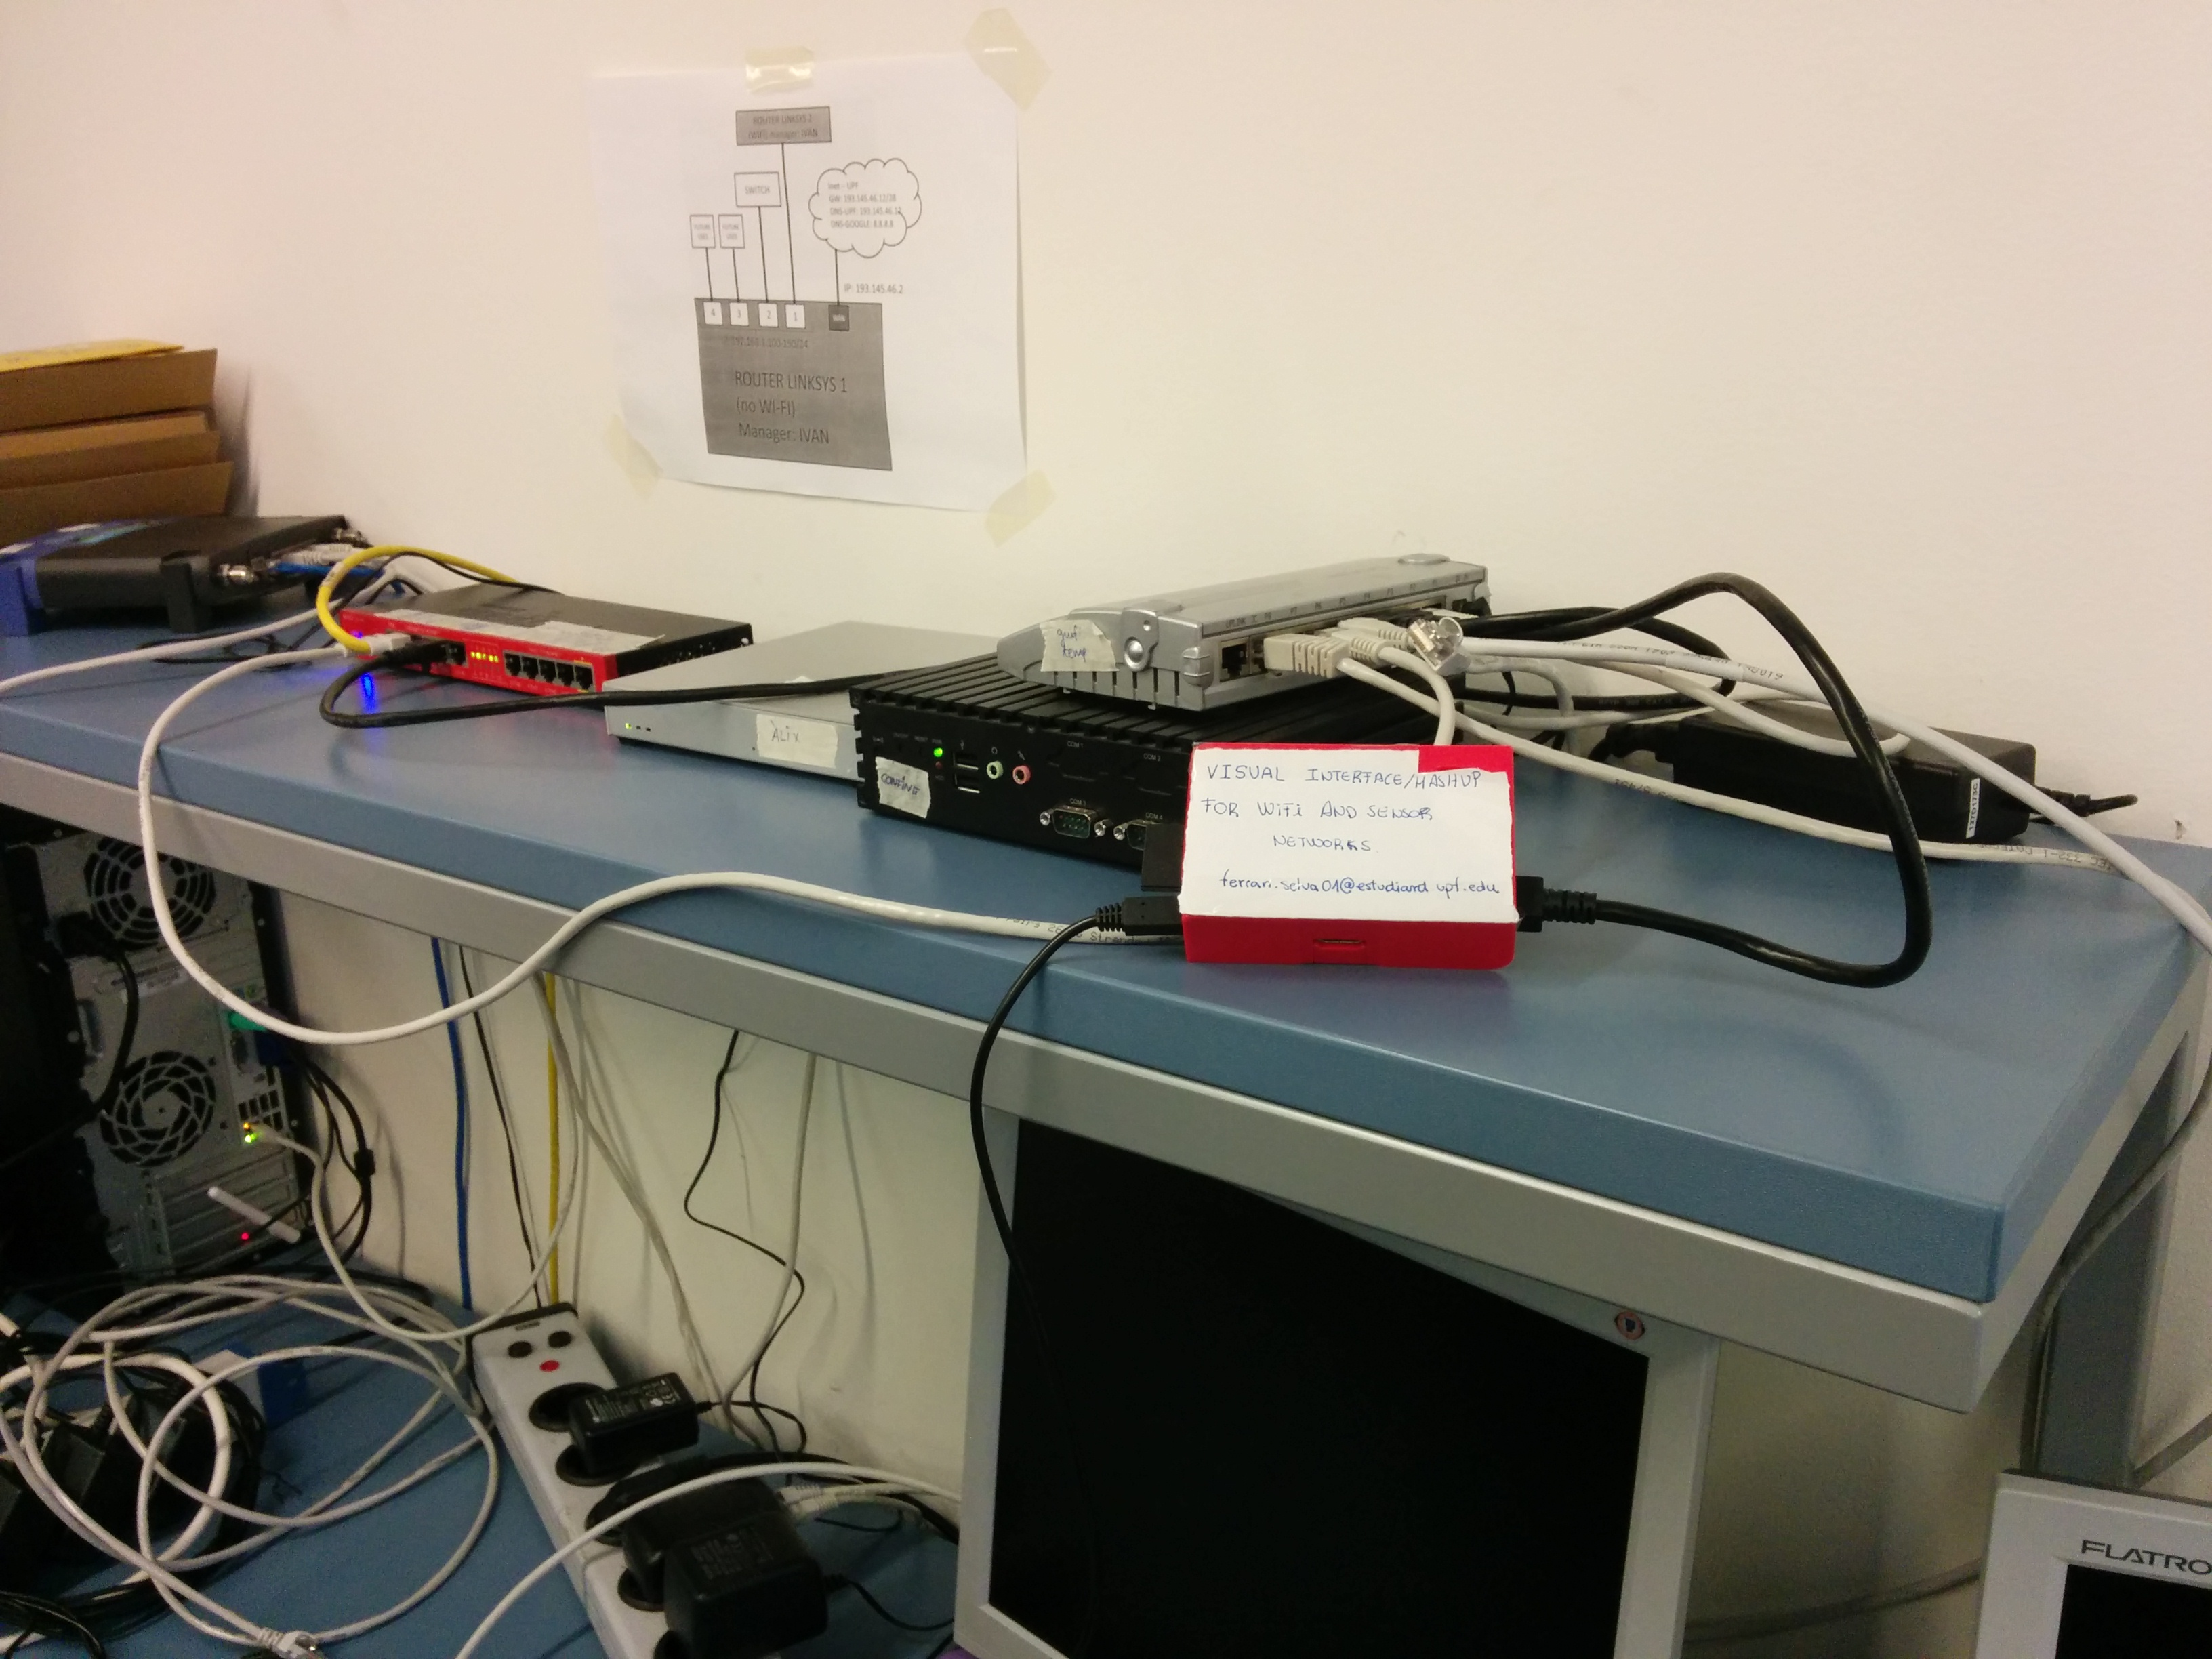
\includegraphics[scale=0.13]{./figures/RaspGuifi.jpg}
              \rule{32em}{0.5pt}
            \caption[Raspberry Pi at Guifi.net Network]{Raspberry Pi at Guifi.net Network}
            \label{fig:snmp}
        \end{figure}
        


 \chapter{TESTING THE SYSTEM}
\label{Chapter5}

The test of the system began the 2014-06-05 at 10:30 and finished the 2014-06-10 at 10:30. During five days, the system has been monitoring the Access Points of the network \emph{Poblenou Sense Fils} in Poblenou district from Barcelona. This network is owned by \textit{guifi.net}. This organization gave the permissionss to carry out the test.

The figures \ref{fg:resumebt} to \ref{fg:dataat}, shows the stats of the collections Resume and Data before and after the test.
    
            \TwoFig{./figures/Resumebt.png}      {Collection Resume Statistics Before Test.}  {fg:resumebt}
       {./figures/Databt.png}{Collection Data Statistics Before Test.}{fg:databt}
       
                   \TwoFig{./figures/ResumeAT.png}      {Collection Resume Statistics After Test}  {fg:resumeat}
       {./figures/DataAT.png}{Collection Data Statistics After Test}{fg:dataat}
        
    
    The fields from the collections to be controlled are:
    \begin{itemize}
    \item Collection Size.
    \item Number of documents.
    \item Document Size.
    \end{itemize}
    
    The relevant stats of the collections are summarized at the table \ref{tab:DBstate}. 

        \begin{table}[H]
        \centering
        \resizebox{15cm}{!}{
\begin{tabular}{c|c|c|c|c|}
\cline{2-5}
                                                   & \multicolumn{2}{c|}{\textit{Before}}            & \multicolumn{2}{c|}{\textit{After}}           \\ \cline{2-5} 
                                                   & \textbf{DataPoblenou} & \textbf{ResumePoblenou} & \textbf{DataPoblenou} & \textbf{DataPoblenou} \\ \hline
\multicolumn{1}{|c|}{\textbf{Collection Size}}     & 0                     & 12.624 Bytes             & 207.0792 Bytes         & 12.944 Bytes           \\ \cline{1-1}
\multicolumn{1}{|c|}{\textbf{Number of Documents}} & 0                     & 45                      & 19.766                 & 45                    \\ \cline{1-1}
\multicolumn{1}{|c|}{\textbf{Document Size}}       & 0                     & 280'53 Bytes            & 104'76 Bytes          & 287'64 Bytes          \\ \hline
\end{tabular}
        }
        \caption{Summary Table of Collections Stats}
        \label{tab:DBstate}
        \end{table}
        
    
    \section{Results}
    The results of the Test are:
    \subsection{Collection Size}
    \textbf{Data Collection}\\
    The Data collection is empty before the start of the test. This is because the Data collection is a register where the documents are stored, with the ID of the access point, the status, and the timestamp of the moment when the checkup is done.
    
    When the system is booted, the Data collection begins to fill with the information gotten of the access points.
    
    At the end of the test, the Data collection had a size of 2.070.792 Bytes. 
    
    This collection is the fastest growing one. That occurs because is the only one that is storing new documents (\textit{Insert}). At the Resume collection, the documents are modified, but new documents will not be added.\\
    
    \textbf{Resume Collection}\\
    The Resume Collection, at start, had a size of 12.624 Bytes.
    At the start of the test, the documents have the IDs, the position and the IPs of the access points. But the remaining fields are initialized with "0".
    
    When the system starts monitoring the network, the fields ``STATUS", ``SINCE", ``TOTALTIME", ``UPTIME", ``DOWNTIME" and ``AVAILABILITY" are modified to the values obtained by the Access program.
    
    At the end, the size of this collection, was of 12.944 Bytes. It increased. But this increase is not significant.

    \subsection{Number of Documents}
    
    The Resume collection, has always the same number of documents.
    While Data collection, will increase its documents number, each iteration by the number of access points to be monitored.
    
    This is the reason why Data collection increased the number of documents in 19.766, while Resume collection remain in 45 documents.
    
    \subsection{Document Size}
    
    Documents from Resume collection has more size because its documents have more fields than Data collection ones. While Data documents will have 3 fields, the Resume documents include 10 fields. 
    The difference between the both collections documents size is of 182'66 Bytes.


    \subsection {Mailing}
Mailing feature has operated correctly. The email address that sends and recieves these alert mails is: {\emph{\href{mailto:bub.project.apcontrol@gmail.com}{bub.project.apcontrol@gmail.com}}.

It has received 223 emails about the stop of different access points and server warnings during the five days that the system was been tested.
    
    For example, the program reported that hotspot with ID: \textbf{BCNgranvia940AH} was down, several times. This mean that the node has been changed its status UP to DOWN and DOWN to UP several times. 
    
    Probably this access point is damaged, and it should be repaired or changed.
    
    The mails received are shown at the figure \ref{fig:mail}.\\
    
        \begin{figure}[htbp]
          \centering
              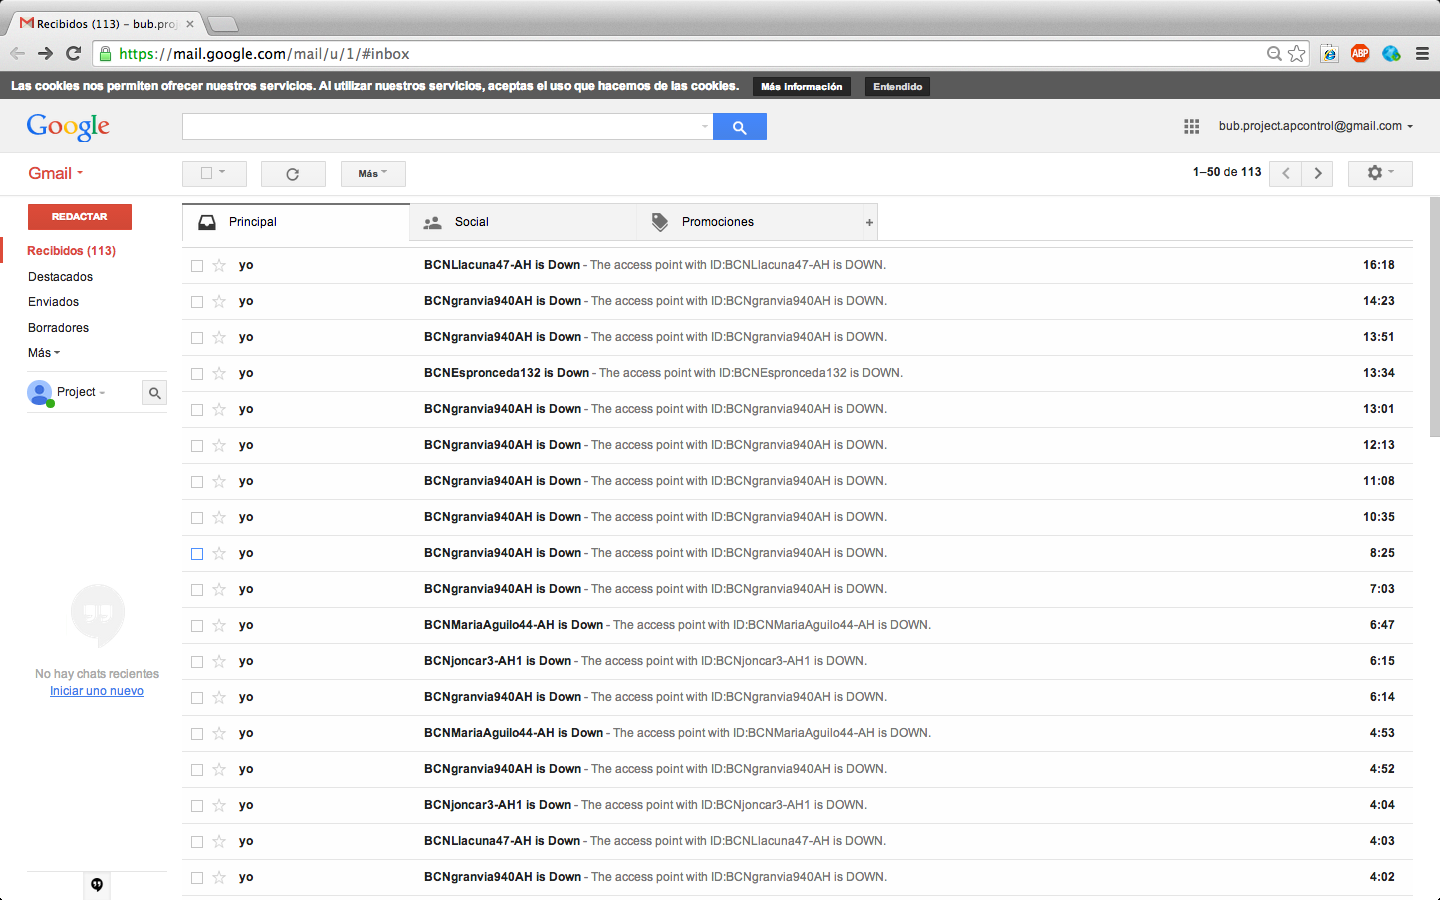
\includegraphics[scale=0.3]{./figures/mails.png}
              \rule{32em}{0.5pt}
            \caption[Mails received when a access point is DOWN]{Mails received when a access point is DOWN}
            \label{fig:mail}
        \end{figure}
    
    \subsection{Web Application}
    The web Application was available all time. The information shown was correct, in the sense that was the same information than the current information stored on the database.
    
    \subsection{Time}
The Access program was executed correctly at the boot of the Raspberry Pi, and the loop that checks, processes, and sends the status of the access points was executed correctly 15 minutes after the last iteration.

    \subsection{Processing the Information}
    
    The process of the information was done correctly. The data that has been checked is:
    
    \subsubsection{TOTALTIME}
    The test of the system started the day 2014-06-05 at 10.30 hours, and finished the day 2014-06-10 at 10.30 hours. This suppose a duration of 120 hours. \\
    
    To check that this is correct, It is needed to get the TOTALTIME of an access point, for example, node with ID: \textbf{BCNgranvia940AH}. Looking to the figure \ref{fig:gv}, the TOTALTIME of this hotspot is 430.977'44 seconds. That means 119'71 hours.
    
    So the system monitored this access point during 119,71 hours, and the test stopped at 120 hours of the start. This little difference is because the last iteration, had not been done when the test finished.
    
    
        \begin{figure}[H]
          \centering
              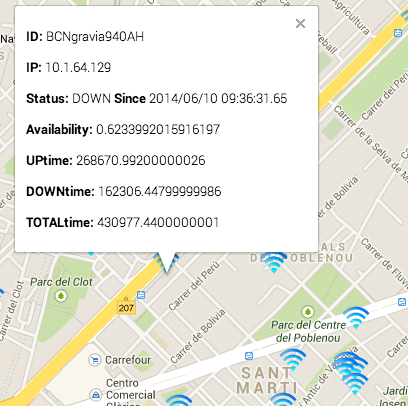
\includegraphics[scale=0.5]{./figures/granviastat.png}
              \rule{32em}{0.5pt}
            \caption[Information of the Access Point \emph{BCNgranvia940AH}]{Information of the Access Point \emph{BCNgranvia940AH}}
            \label{fig:gv}
        \end{figure}
    
    
    \subsubsection{AVAILABILITY}
    To calculate the availability, the Access program divides UPTIME between TOTALTIME. 
    To check this result, using the node \emph{BCNgranvia940AH} shown at the figure \ref{fig:gv}, the result of divide 268.670'992 by 430.977'44 is 0'623399. This is the same value of the shown in the figure. So this feature operated correctly.
    
    \subsection{Unexpected stops}
    There were no unexpected stops during the five days that the system was being tested.
Anyway, the system stop should not be a problem, because restart the system is easy. Just rebooting the Raspberry Pi, the access program should be executed automatically, and continue monitoring the access points of the network. No action is required at the database, to follow working properly.
    
    \subsection{Warnings Reported}
    There is one warning reported. This warning is:
    
    \paragraph{apache2: Could not reliably determine the server's fully qualified domain name, using cfe-nets.s.upf.edu for ServerName}.
    
    It is not an error. It happens when the \textit{apache2} does not know the Domain Name System server\footnote{The Domain Name System, or DNS, is a system that provides a distributed database, that store the names assigned to the devices and services on the network. These names are called Domain Names \cite{DNS}.}. It is not important for the right operation of the system.
    
    \section{Collaboration with other Organizations}
    
    The project started with the collaboration of the Institut Municipal d'Informàtica (IMI), but the communication with this institution was complicated. The IMI is a big institution, and hold the communication was difficult.
    
    The testing of the system at IMI's network could not be performed due not having the IPs of the access points of BarcelonaWi-Fi.
    
    For test the system, emerged a new organization, called Guifi.net. This institution, gave permission for the test of the system using its network \emph{Poblenou Sense Fils} located at Poblenou district in Barcelona.} 
    
    The communication with this institution was easier, and the fact that its network has a node at the Universitat Pompeu Fabra, was helpful when the system was being tested. 
    
    
\chapter{CONCLUSIONS}
\label{Chapter6}

This project shows that is possible to implement a inexpensive system to monitor the Access Points of a determined network. This will not give a full knowledge of the access points status, but will give some valorous information.

The system is composed by a Raspberry Pi and a Server. The Raspberry Pi is hosting a program made in java to get information about the access points. The server, is used to host the web application, the web service, and the MongoDB database. The web application displays the information stored at the database, and the web service is used for the information exchange between the Raspberry Pi and the server. Finally, the Database stores the information gotten by the program at Raspberry Pi.

The system has been tested during five days. The information recollection has operated correctly. There has not been problems with the web application. The emails were sent at the correct moment, with the correct content. In summary, the results of the test show a good performance of the system.

The system is simple, this allows the correct operation for all networks just knowing the IP Addresses of the hotspots. On the other hand, there is a lot of information that could be interesting to know that is being lost.






\chapter{FUTURE WORK}
\label{Chapter7}

A project of this type can be developed in many ways. With the work done so far, it is possible to control whether the access points are in operation or not, whether the hotspots are stopped rarely or usually, its availability and more data, but it could still add more benefits to this system.

For improving the capacity of obtaining or picking up information, the SNMP\footnote{Simple Network Management Protocol (SNMP): Protocol used to communicate management and control information between the network management stations and the agents in the network elements. The agent is the software, located on the managed device, that gets information available and translate it a supported SNMP format. The network management stations are the devices that process the information and control the managed devices \cite{SNMP}.} protocol, can be useful. To add SNMP queries would give access to important new information as the number of connected users in real time. This incorporation also, opens new possibilities, in the sense that the system, for the moment, is only monitoring the access points. With this addition, it would be possible to, also, control these hotspots. This control capability gives the chance of new features, like turn on, turn off, reboot and among many others, the controlled hotspots, remotely.

SNMP scheme about its operation is shown at the figure \ref{fig:snmp}.\\

It is possible to integrate SNMP queries to java codes. There are libraries like \textit{snmp4j}. This open source library, provides the needed classes and interfaces for the creation of SNMP messages, and its communication \cite{snmplibrary}.

So, this options is something to be considered. The Access program could execute the code to use this protocol. The hardware and software of the system can support this protocol too. The only question is if all the access points will support this protocol and which version of it. 

There are compatibility problems between different versions of SNMP. This is something that should take into account if there is the intention of deploy this protocol to the system.

Moreover, it could be improved the interface of the web application. Nowadays, it is displayed the map with Access Points and the available information. To this information, it could be added features like, view the log of a particular access point, or add search options like search an access point by status, area or fewer users.

     \begin{figure}[htbp]
          \centering
              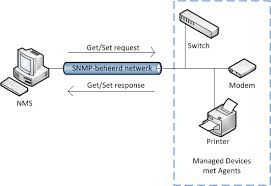
\includegraphics[scale=1]{./figures/snmp.png}
              \rule{32em}{0.5pt}
            \caption[SNMP Scheme]{SNMP Scheme}
            \label{fig:snmp}
        \end{figure}

\addcontentsline{toc}{chapter}{Bibliography}
\bibliography{bibliography}
\cleardoublepage

\appendix
\label{appendix}

  \chapter{Pilot Charter}
  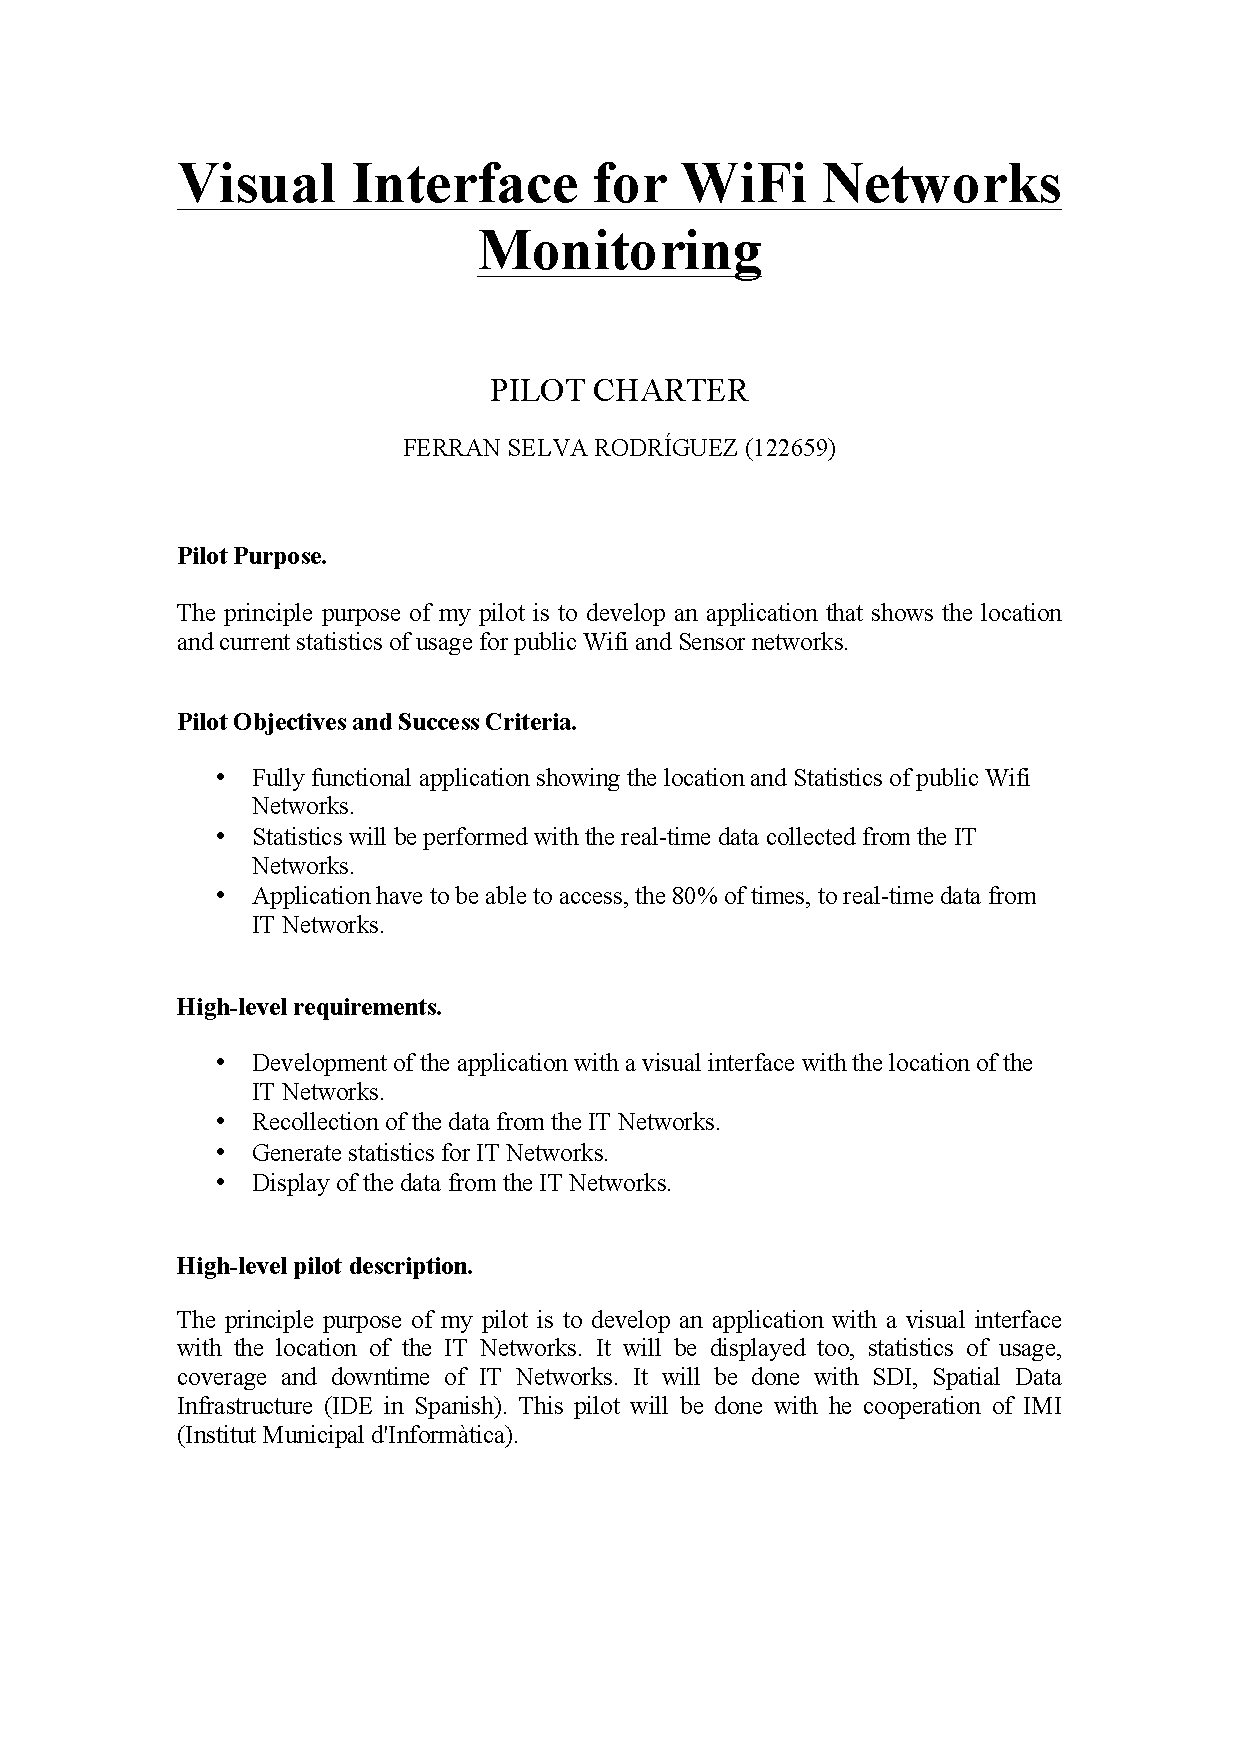
\includepdf[pages={1,2}]{PilotCharter.pdf}
  \chapter{Gantt Diagram}
  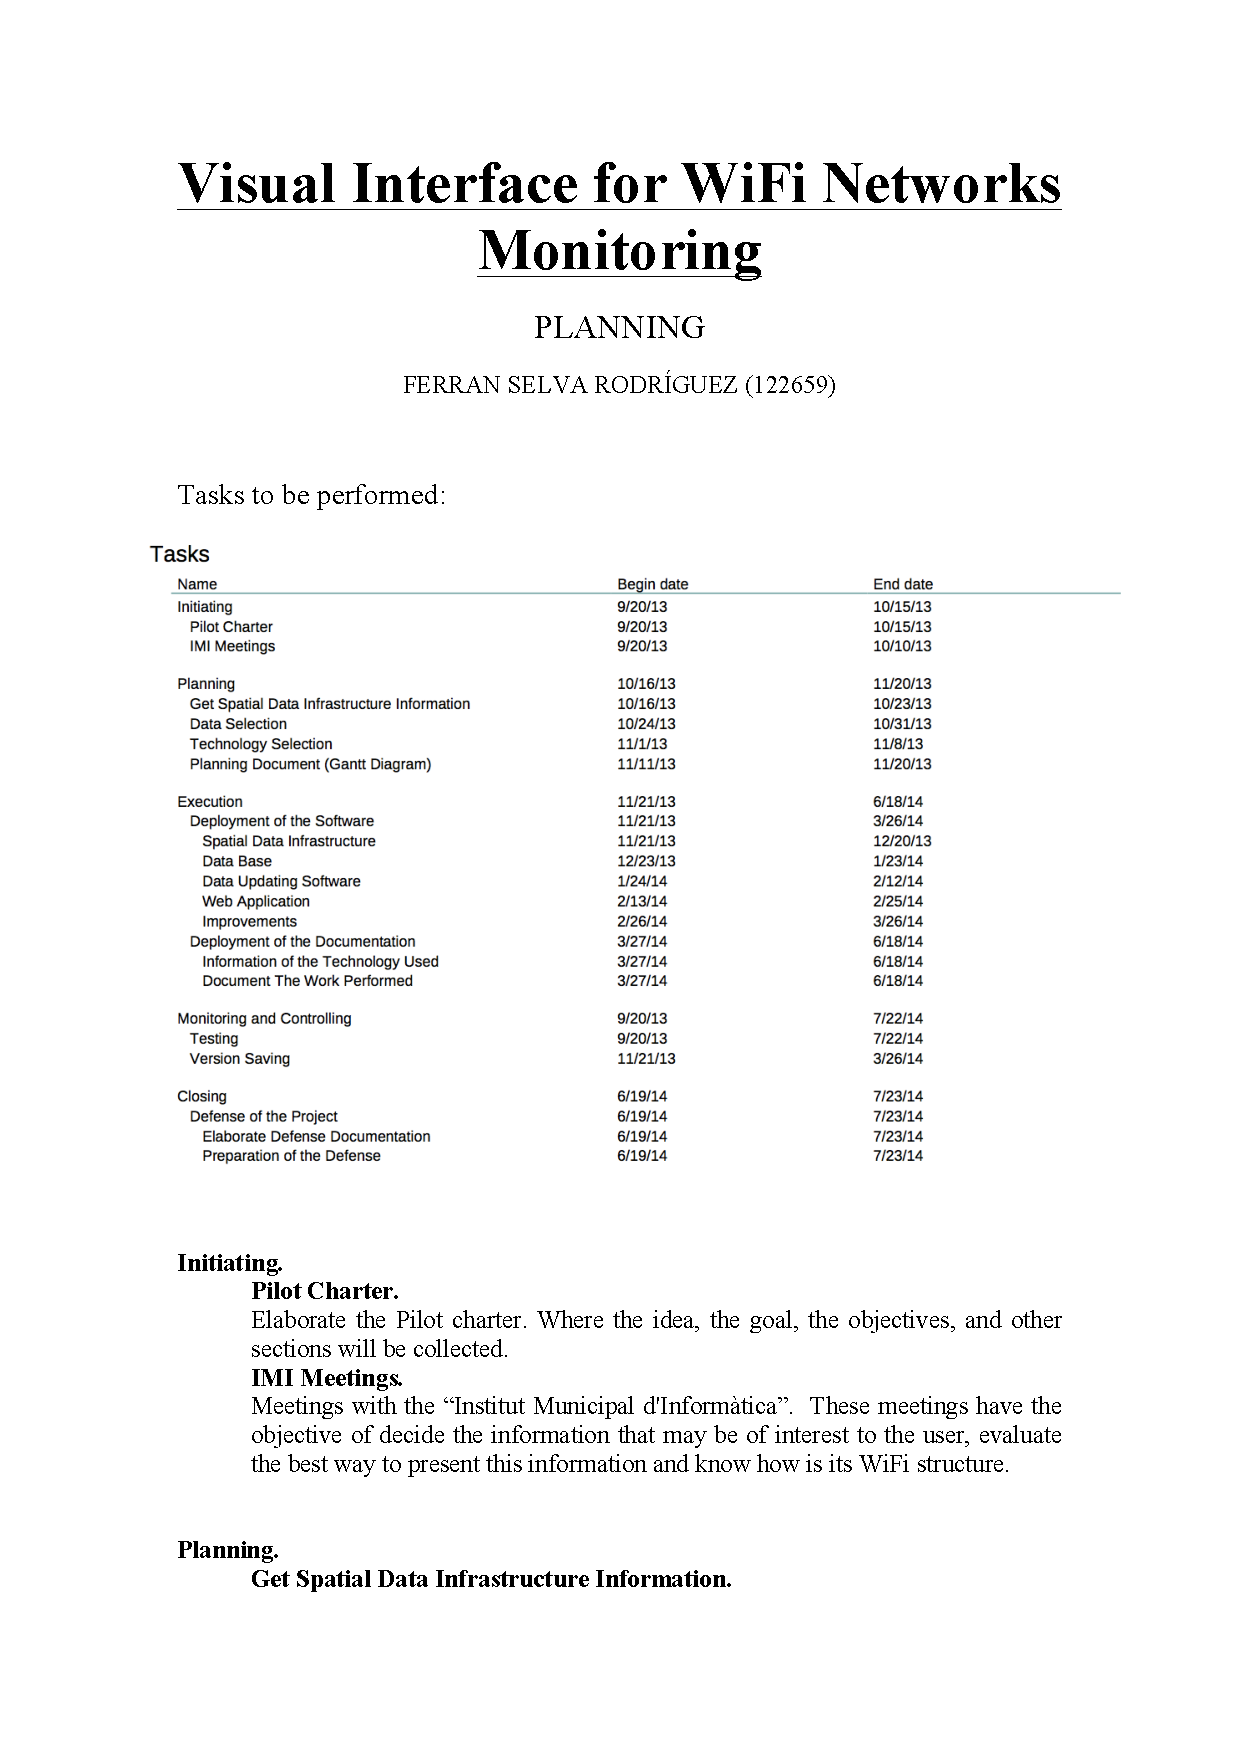
\includepdf[pages={1,2,3}]{Planning.pdf}
  


\backmatter
\printindex





\end{document}


%NUMERACIÓ DE LA PÀGINA EXTERIOR EXCEPTE EN LA PRIMERA PÀGINA DE CADA CAPÍTOL
\usepackage{fancyhdr}
\pagestyle{fancy}
\fancyfoot{}
\fancyfoot[RO]{\thepage}
\fancyfoot[LE]{\thepage}


%MUTIPLES ÍNDEX
%En el preàmbul
\usepackage{multind}
\makeindex{authors}
%Introducció d'entrades la forma
\index{authors}{Einstein}
%Situació de l'Índex
\printindex{authors}{Author index}
%Cal eliminar les comandes \usepakage{makeidx} \makeindex \printindex
%cal exacutar des de la línia de comandes makeindex authors
